\chapter{Middlemen as entrepreneurs}
\label{ch:criticalnodes}

Research has recognised networks as important descriptors of social and economic processes \citep{Watts2004,Jackson2008,Newman2010}. The outcome of the agent-based simulations in Chapter~\ref{ch:relationaltheory} showed that as the networked interaction infrastructure develops the set of economic interactions and relationships can form an irregular topology where individual agents hold heterogeneous positions in the infrastructure. As a consequence of their interactions some economic agents hold more `central' positions in the infrastructure than others: the centrality of individual economic agents is distributed unevenly across the network. We noted in the previous chapter that the formation of a new socio-economic role through entrepreneurial effort comes with it the formation of a unique set of economic interactions and thus a unique position in the socio-economic space. The unique position of individual agents is closely related to the discussion of the middleman here.

This chapter makes a contribution to the analysis of economic agents, depicted generally as nodes, that are critical for the flow of information and trade in a network. Such critical agents---or ``middlemen''---have been solely considered for undirected networks. Here, we consider these nodes in the more general context of directed networks. We introduce a middleman as a specific type of node that can block the information flow from at least one node to another. If one applies this definition to undirected networks, one arrives at the standard notion of a middleman as a singleton node cut set. In the context of directed networks this is no longer the case: Its removal does not necessarily break up the whole network; it just compromises the information flow for at least one pair of nodes. In networked economies, the essential brokerage position of middlemen allows them to be highly extractive to both directly and indirectly connected nodes. On the other hand, their involvement lowers transaction costs in terms of search and the formation of beneficial links \citep{Burt1992}.

Naturally, the existence of middlemen is closely related to the competitive environment represented by that network. \citet{GillesDiamantaris2013} show in a very simple setting that middlemen have the potential to be highly exploitive given a lack of competition combined with a pessimistic outlook regarding their potential contestability in a network. The main conclusion from this research is a non-trivial extension of how economists and social scientists perceive the architecture and dynamics of exchange systems, how the presence of a middleman can knit a system together, and, as a consequence of their position, can act as rent-extracting monopolists with excessive bargaining power \citep[Chapter~11]{EasleyKleinberg2010}.

We extend these notions to a more general definition of contestability in directed networks. In a directed network, a node is contested if alternative pathways are available to establish exchange between pairs of nodes in the network. Our main result shows that there is a formal duality between the existence of middlemen and network contestability. In particular, an intermediary node is a middleman if and only if it is uncontested.

One would expect that betweenness centrality measures would capture the influence that such middlemen exert. However, we show that this is not the case. Instead, we propose a new \emph{middleman power measure} that exhibits the desired properties. We devise an algorithm that applies the adjacency matrix of any directed network to identify and measure the middlemen in that network. We apply this algorithm to study two very well known (historical) directed networks from the literature. These applications allow us to make an in-depth comparison with well-established centrality measures such as betweenness centrality and Bonacich centrality \citep{Bonacich1987}.

In the Florentine marriage network of the early renaissance \citep{Padgett1993,Padgett1994}, we conclude that our middleman power measure clearly ranks the more powerful middlemen higher than the less powerful, confirming with historical analysis. In \citet{Krackhardt1987}'s advice network, again our measure confirms Krackhardt's original assessment of the most influential node. Furthermore, we show that, despite the importance of middlemen in these networks, this positional feature is not properly and fully identified by conventional centrality measures.

\paragraph{Middlemen as entrepreneurs.}

In complementing our claim regarding the relationship between middlemen and competition, we consider middlemen as entrepreneurs. Middlemen are regarded as economic agents that form a new socio-economic role and therefore possess a unique position within society; they connect to otherwise disconnected agents and gain from the bridging of communities and the integration of ideas and specialisations.

We note that the economic state of the Platonian economy is used throughout the assessment of the next two chapters; and as such we concentrate on the existence of a horizontal division of labour\footnote{However, some easy extension can be made to capture phenomena in more vertical divisions of labour.}. The horizontal division of labour allows for the production of relatively complex consumption goods, which are only realised through a sequence of intermediate stages performed by distinct individuals. This is exactly what is depicted throughout this chapter as we consider such concepts as \emph{contestability} in networks. From the flow of exchange through intermediation, some economic agents may be considered as more powerful and influential than other agents. \emph{Node centrality} can help to identify the most influential economic agents in the socio-economic space.

\subsubsection{Standard measures of node centrality}

Middlemen have been investigated in both sociology and economics during the past three decades. The specific interest in economics was initiated by \citet{KalaiMiddlemen1978} who investigated the payoffs to middlemen in an intermediated trade environment. These insights were extended by \citet{RubinsteinWolinsky1987} who applied them to a model of market search. \citet{JacksonWolinsky1996} and \citet{GillesChakrabarti2006} further analysed middlemen in the context of economic interaction.

Many of the general findings in the economics literature have been independently verified in the social sciences. In social network analysis, middlemen are seen as social actors that bridge structural holes in the social fabric. Due to their position these middlemen have access to more diverse information; are able to broker information and ideas between agents and affiliations; will have a tendency to be more entrepreneurial; are able to exploit their intermediating opportunities; and have better ideas which are then evaluated by others within a society or organisation \citep{Burt1992, Burt2004,Burt2005,Burt2010}. Moreover, by virtue of their weak ties in the network, middlemen are able to exploit unique opportunities that are not afforded to other, more socially embedded, nodes in the network \citep{Granovetter1973, Granovetter2005}.

Despite the wide acknowledgement within social network analysis of the significance of middlemen, centrality measures do not necessarily identify these critical nodes as being important even though their removal may deteriorate the functionality of the network as a whole. As the notion of centrality came to the fore, \citet[p.~219]{Freeman1979} argued that central nodes were those ``in the thick of things''. To exemplify this, he used an undirected star network consisting of five nodes. The middle node, at the centre of the star, has three advantages over the other nodes: It has more ties; it can reach all the others more quickly; and it controls the flow between the others. Freeman developed three simple measures of node centrality based on the prevalent features of the center node: degree, closeness and betweenness.

More complex centrality measures have been proposed. \citet{Bonacich1972,Bonacich1987,Bonacich2001} proposed the use of the largest eigenvalue of the adjacency matrix as the basis for the measurement of network centrality. This measure expresses the idea that a node is more central if it is connected to nodes that are themselves central. Other measures, including Katz centrality \citep{Katz1953} take advantage of the same mechanism as Bonacich centrality by analysing the number of all nodes that a given node can be connected through a path, while contributions from linking distant nodes are progressively penalised. A node has a larger centrality if it has neighbours with a high Katz centrality. PageRank \citep{BrinPage1998} is a variant of Katz centrality, which recently gained application to the World Wide Web. Moreover, these common measures of centrality have been applied to many different social and economic contexts, and have had application to directorate networks (Khanna et al., 2015; El-Khatib, 2015).

The most common centrality measures do not provide a proper account of network power and, usually, overlook middlemen. Two exceptions are noted: First, the $\beta$-measure \citep{BrinkGilles1996, BrinkGilles2000} is founded on an axiomatic approach to measuring centrality. This measure is one of a few that measures dominance, and therefore power, in directed networks. \citet{BormBrink2002} develop an iterated $\beta$-measure which, much like the eigenvector and PageRank centralities, develops a score based on the dominance of the nodes that it dominates. Again, this lacks a specific application to directorate networks. Applications are mainly focussed on how nodes are dominated by others in hierarchical organisations. Second, \citet{Bozzo2015} provide both a vulnerability and power measure based on the number of nodes that can be victimised by so-called ``executioners''. The power of a node set is comparable to how integral the set is to the robustness of an undirected network.

\paragraph{Chapter outline.}

This chapter is partitioned into four sections. The first provides the required preliminaries for our analysis and introduces strong and weak middlemen within networked socio-economic spaces. We also consider the notion of network contestability, which is shown to be the dual notion to that of middlemen. The second section discusses a measure of middleman power, which assigns a quantitative expression to a node's brokerage power. The third section provides a variety of measures in which to assess the competitiveness of a network in both a static and dynamic sense. The final section investigates two empirical case studies of social networks where middlemen have tended to have importance: the Florentine marriage network and Krackhardt's advice network.

\section{Middlemen and contestability}

Our initial discussion focuses on the definition of a critical nodes in a directed network, which we denote as \emph{middlemen}. We introduce middlemen in relation to the connectivity in a network. In doing so we identify two related notions of middlemen, denoted as strong and weak middlemen depending on their network position.

\subsection{Preliminaries}

We formally defined a socio-economic space as a set of economic interactions between a population of consumer-producers or economic agents, the result of which forms a network of relations. This definition infers that all social and economic interaction is two-way and thus symmetric. In reality, not all interactions and relationships are bilateral; especially when considering the flow of intermediate goods or information in a network. This distinction between symmetric and asymmetric relationships can be represented by undirected and directed relationships.

\paragraph{Directed and undirected networks.}

The network that is described through the formal definition of a socio-economic space is considered as an \emph{undirected network} such that all interactions are symmetrical. For example, given an undirected relationship between two agents, both agents can interact with each other. Many fundamental social and economic engagements can be considered in this symmetric manner.

A more generalised version of an undirected network is a \emph{directed network} which consists of directed relationships. A directed relationship between two agents is considered asymmetric such that one agent can interact with the other, but this interaction is not reciprocated. We note that a directed relationship is more general than an undirected relationship because a reciprocated directed relationship leads to an undirected relationship. Directed relationships and networks are also useful to describe social and economic networks. Specifically they can be used to describe the flow of information and economic goods and commodities within social and economic relationships.

We analyse social and economic interactions in terms of a set of directed relationships that forms a directed network. A directed network is a pair $(N,D)$ where $N = \{1,2, \ldots ,n\}$ is a finite set of economic agents, or \emph{nodes}, and $D \subset \{ (i,j) \mid i,j \in N$ and $i \neq j \}$ is a set of \emph{arcs}, being directed relationships from one node to another. Note that $(i,i) \notin D$ for any $i \in N$, which is a technical requirement\footnote{An \emph{undirected} network can be interpreted as a directed network $(N,D)$ such that all arcs are reciprocated: $(i,j) \in D$ if and only if $(j,i) \in D$.}. We denote a directed network $(N,D)$ by $D$ unless $N$ is ambiguous. Also, we denote $(i,j) \in D$ by $ij$. We next introduce some auxiliary concepts in directed networks.

\paragraph{Walks.}

A \textit{walk} from $i$ to $j$ in a directed network $D$---or, simply, a $(i,j)$-\emph{walk}---is a set of connected nodes $W_{ij} (D) = \{ i_{1}, \ldots ,i_{m} \} \subset N$ with $m \geqslant 3$, $i_1 =i$, $i_m =j$, and $i_{k}i_{k+1} \in D$ for every $k=1, \ldots ,m-1$. Therefore, a walk is a sequence of adjacent nodes in the network. Walks might revisit nodes and, therefore, might contain loops.

In many cases there are multiple walks from $i$ to $j$ in a directed network $D$. If this is required, we denote $W_{ij}^{v}(D)$ as the $v^{\mbox{th}}$ distinct walk from $i$ to $j$ in $D$.

The class $\mathcal{W}_{ij}(D)= \{ W_{ij}^{1}(D), \ldots ,W_{ij}^{V}(D) \}$ consists of all distinct walks from $i$ to $j$ in $D$, where $V$ is the number of distinct walks. $\mathcal{W}_{ij}(D)= \varnothing$ denotes that there is no walk from $i$ to $j$ in $D$.

\paragraph{Connectedness.}

Nodes $i,j \in N$ are \textit{strongly connected} if $\mathcal{W}_{ij}(D) \neq \varnothing$ as well as $\mathcal{W}_{ji}(D) \neq \varnothing$. A directed network $D$ is \emph{strongly connected} if $\mathcal{W}_{ij} \neq \varnothing$ and $\mathcal{W}_{ji} \neq \varnothing$ for all nodes $i,j \in N$.

Node $i$ is \textit{weakly connected to} $j$ if $\mathcal{W}_{ij}(D) \neq \varnothing$. A directed network $D$ is weakly connected if for all $i,j \in N$ either $i$ is weakly connected to $j$, or $j$ is weakly connected to $i$, or both. Clearly, strongly connected networks are always weakly connected.

A subset $M \subset N$ is a \emph{weakly connected component} of $D$ if $(M, D_M)$ with $D_M = D \cap (M \times M)$ is weakly connected and and there is no $i \in N \setminus M$ with $(M+i, D_{M+i})$ being weakly connected.

\paragraph{Successors and predecessors.}

If $\mathcal{W}_{ij} (D) \neq \varnothing$ then $j$ is called the \textit{successor} of $i$ and $i$ is called the \textit{predecessor} of $j$ in $D$.

For $i \in N$ we define $s_{i}(D) = \{ j \in N \mid (i,j) \in D \}$ being all of the \textit{direct successors} of $i$ in $D$, and $p_{i}(D)=\{j \in N \mid (j,i) \in D\}$ being all the \textit{direct predecessors} of $i$ in $D$. The \emph{out-degree} of $i$ is given by $d_{i}^{+} = \# s_{i}(D)$ and its \emph{in-degree} by $d_{i}^{-}= \# p_{i}(D)$. Now, $i$'s overall degree is given by $d_{i} = \# \{ s_{i} (D) \cup p_{i} (D) \}$.

We also use $P_{i}(D)=\{j \in N \mid \mathcal{W}_{ji}(D) \neq \varnothing \}$ which denotes $i$'s \textit{predecessor set}, and $S_{i}(D)= \{j \in N \mid \mathcal{W}_{ij}(D) \neq \varnothing \}$ being $i$'s \textit{successor set}\footnote{We emphasise that we do not include $i$ in its own predecessor or successor set.}. Node $k$ is an \emph{indirect successor} of $i$ in $D$ if $k \in S_{i}(D) \setminus s_i (D)$ meaning that $\mathcal{W}_{i,k}(D) \neq \varnothing$. Thus, $i$'s successor set includes all of $i$'s direct and indirect successors.

Likewise, node $k$ is an \emph{indirect predecessor} of $i$ in $D$ if $k \in P_{i}(D) \setminus p_{i}(D)$, i.e., $\mathcal{W}_{k,i}(D) \neq \varnothing$. $i$'s predecessor set consists of all of $i$'s direct and indirect predecessors.

\begin{definition}[Origin and reach] \label{coverage}
Consider a directed network $(N,D)$ and a node $i \in N$.
\begin{itemize}
\item The \textbf{origin} of node $i$ denotes the fill set of $i$'s predecessors including node $i$
\begin{equation}
\overline{P}_{i}(D) = P_{i}(D) \cup \{i\}.
\end{equation}
\item The \textbf{reach} of node $i$ denotes the fill set of $i$'s successors including node $i$
\begin{equation}
\overline{S}_{i}(D) = S_{i}(D) \cup \{i\}.
\end{equation}
\end{itemize}
\end{definition}

The node set $N$ can be partitioned into three disjoint subsets: sources, sinks, and intermediaries. Node $i$ is a \emph{source} if $d_{i}^{-} = 0$ and $d_{i}^{+} \geqslant 1$; $i$ is a \emph{sink} if $d_{i}^{-} \geqslant 1$ and $d_{i}^{+} = 0$; and $i$ in an \emph{intermediary} if $d_{i}^{-} \geqslant 1$ and $d_{i}^{+} \geqslant 1$.

Finally, we let $i \in N$ and $D-i$ be equivalent to:
\begin{equation}
D - i = D_{N \setminus i} = \left\{ (j,h) \in D \mid j,h \in N \setminus i \right\} .
\end{equation}

Therefore $D_{N \setminus i}$ is the restricted network that removes all nodes in node set $i$ and all arcs to and from the nodes in $i$.

\subsection{Connectivity and middlemen}

We identify \textit{critical nodes} as those having the ability to broker information flows in a network. Following \citet{GillesChakrabarti2006}, a critical node in an undirected network can disrupt and manipulate the typical operations on a network by disconnecting two or more nodes---which is equivalent to the property that removing a critical node partitions a given network into multiple disconnected components.

Here, we extend this concept to directed networks. In this context our definition focusses on the disruption of connectivity of two nodes.

\begin{definition}[Middleman] \label{middleman}
Let $D$ be a network on node set $N$, where $h \in N$.
\begin{itemize}
\item Node $h$ is an \textbf{$(i,j)$--middleman} if for some pair $i,j \in N$ $\mathcal{W}_{ij} (D) \neq \varnothing$ and
\begin{equation} \label{ijmiddleman}
h \in \bigcap \mathcal{W}_{ij}(D) \setminus \{i,j\} = W_{ij}^{1}(D) \cap  \ldots  \cap W_{ij}^{V}(D) \setminus \{i,j\},
\end{equation}
where $V \geqslant 1$ is the number of walks from $i$ to $j$. Here, $M_{i,j}(D) \equiv \cap \mathcal{W}_{ij}(D)$ denotes the \textbf{$(i,j)$--middleman set} containing all $(i,j)$--middlemen.

\item The \textbf{middleman set} for $D$ is the set of all middlemen in $D$ given by
\begin{equation} \label{middlemanseteq}
M(D) = \bigcup_{i,j \in N \colon i \neq j} M_{i,j}(D)
\end{equation}
Node $h$ is a \textbf{middleman} if $h \in M(D)$ and $h$ is a \textbf{non-middleman} if $h \notin M(D)$.
\end{itemize}
\end{definition}

A middleman is an intermediary node that is a member of \emph{all} walks between at least two other nodes within a given network. Therefore, a middleman brokers the flow of all information between at least two nodes. Obviously, a middleman connects two or more agents that would not be connected otherwise. Indeed, by definition $M_{i,j} (D) \neq \varnothing$ if and only if $\mathcal{W}_{ij} (D) \neq \varnothing$.

Converse to a middleman, a non-middleman is an intermediary that if removed from the network does not affect the connectivity of any two or more other nodes and, therefore, does not impose a negative externality on other nodes when removed.

The following properties can be deduced directly from the above definition.

\begin{proposition}\label{TheoremIntermediary}
Let $D$ be a directed network on the node set $N = \{ 1, \ldots ,n \}$.
\begin{itemize}
\item[(i)] Every middleman $i \in M(D)$ is an intermediary in $D$. 

\item[(ii)] If $n < 3$, there might exist intermediaries, but there are no middlemen.

\item[(iii)] For $n \geqslant 3$ and $i \in N$, $p_{i}(D) \subset \left[ p_{j}(D) \cup \{ j \} \, \right]$ for every direct successor $j \in s_{i}(D)$ implies that $i \notin M(D)$.

\item[(iv)] For all $i,j \in N$ with $j \in s_{i}(D)$ it holds that $M_{i,j}(D) = \varnothing$.
\\
This implies that the complete directed network has no middlemen.

\item[(v)] Every middleman $i \in M(D)$ has a local clustering co-efficient of less than $1$.

\item[(vi)] If $D$ is undirected in the sense that $(i,j) \in D$ if and only if $(j,i) \in D$, then $M_{ij} (D) = M_{ji} (D)$ for all $i,j \in N$.
\end{itemize}
\end{proposition}

From (vi), in an undirected network a node is a middleman if it rests on all walks from node $i$ to node $j$. This means that the removal of a middleman disrupts the any communication between nodes $j$ and $i$. Hence, a middleman indeed is a singleton cut set in an undirected network, as traditionally understood.

On the other hand, in a directed network, a middleman rests on all walks from node $i$ to node $j$, but does not have to rest on all walks from $j$ to $i$. This implies that given the removal of a middleman in a directed network the interaction from $i$ to $j$ will become disconnected, but the interaction from node $j$ to node $i$ may still be present. Indeed, even with the removal of a middleman in a directed network, nodes $i$ and $j$ can still remain weakly connected. This insight motivates a further refinement of the notion of a middleman in a directed network.

\begin{definition}[Strong and weak middlemen] \label{strongweakmiddlemen}
Let $D$ be a weakly connected directed network on node set $N = \{ 1, \ldots ,n \}$ with $n \geqslant 3$.
\begin{itemize}
\item A middleman $h \in M(D)$ is a \textbf{strong middleman} in $D$ if the network $D - \{h\}$ contains two or more weakly connected components.

\item A middleman $h \in M(D)$ is a \textbf{weak middleman} in $D$ if network $D - \{h\}$ does not contain two or more weakly connected components.
\end{itemize}
\end{definition}

Weak middlemen exist in both cyclic and acyclic directed networks. Example~\ref{identifyingmiddlemen} highlights the existence of both weak and strong middlemen in an acyclic network.

\begin{figure}[t]
\begin{center}
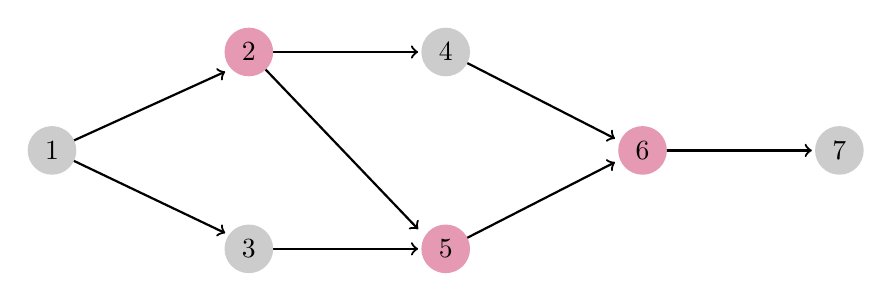
\begin{tikzpicture}[scale=0.5]
\draw[thick, ->] (0,2.5) -- (4.4,4.5);
\draw[thick, ->] (0,2.5) -- (4.4,0.4);
\draw[thick, ->] (5,5) -- (9.3,5);
\draw[thick, ->] (5,0) -- (9.3,0);
\draw[thick, ->] (5,5) -- (9.3,0.5);
\draw[thick, ->] (10,5) -- (14.3,2.8);
\draw[thick, ->] (10,0) -- (14.3,2.2);
\draw[thick, ->] (15,2.5) -- (19.3,2.5);

\draw (0,2.5) node[circle,fill=black!20] {$1$};
\draw (5,5) node[circle,fill=purple!40] {$2$};
\draw (5,0) node[circle,fill=black!20] {$3$};
\draw (10,5) node[circle,fill=black!20] {$4$};
\draw (10,0) node[circle,fill=purple!40] {$5$};
\draw (15,2.5) node[circle,fill=purple!40] {$6$};
\draw (20,2.5) node[circle,fill=black!20] {$7$};

\end{tikzpicture}
\end{center}
\caption[Acyclic directed network highlighting strong, weak, and non-middlemen]{Acyclic directed network, $D$, highlighting strong, weak, and non-middlemen}
\label{weakmm}
\end{figure}

\begin{example} \label{identifyingmiddlemen}
Consider a directed network $D$ on the node set $N=\{1,2,3,4,5,6,7\}$, which is depicted in Figure~\ref{weakmm}. We can determine that $M(D)=\{2,5,6\}$, where nodes 2 and 5 are weak middlemen and node 6 is a strong middleman. For an explanation first consider node 2. Node 2 lies on all walks from node 1 to node 4, therefore $2 \in M_{1,4}(D)$ and $\mathcal{W}_{1,4}(D - \{2\}) = \varnothing$. However, $D - \{2\}$ remains weakly connected meaning that node 2 must be a weak middleman. An analogous argument could be made for node 5 because $5 \in M_{3,6}(D) \cap M_{3,7}(D)$ and, therefore, $\mathcal{W}_{3,6}(D - \{5\}) = \mathcal{W}_{3,7}(D - \{5\}) = \varnothing$. Moreover, $D - \{5\}$ is weakly connected.

Finally, $6 \in M_{1,7}(D) \cap M_{2,7}(D) \cap M_{3,7}(D) \cap M_{4,7}(D) \cap M_{5,7}(D)$. Indeed, node 6 is the sole broker of all interaction to node 7. In the network $D - \{6\}$ there emerge two weakly connected components: $\{ 1,2,3,4,5 \}$ and $\{ 7 \}$.

All other intermediaries are non-middlemen. Indeed, even the removal of either node 3 or 4 does not affect the connectivity in the network\footnote{It is worth noting that if all arcs were reciprocated in network $D$ from Figure~\ref{weakmm} to form an undirected network, nodes 2 and 5 would no longer be middlemen. However, node 6 would still be a strong middleman and would subsequently broker twice as many interactions, i.e. all connections to node 7 and all connections from node 7 to the rest of the network.}.
\end{example}

Theorem~\ref{undirectedmiddlemen} below naturally leads from the insights resulting in Definition~\ref{strongweakmiddlemen} and Example~\ref{identifyingmiddlemen}.

\begin{theorem} \label{undirectedmiddlemen}
Every middleman in an undirected network is a strong middleman.
\end{theorem}

\begin{proof}
Without loss of generality we can restrict ourselves to connected undirected networks only. First note that every connected undirected network is a strongly connected directed network $D$ with $ij \in D$ if and only if $ji \in D$ and there exists at least one walk from $i$ to $j$ for all $i \neq j$.
\\
Therefore, consider a strongly connected directed network $(N,D)$ where $\# N =n \geqslant 3$. According to Definition~\ref{middleman}, a node $h \in N$ is a middleman if it rests on all walks between at least two other nodes, say $i$ and $j$. Since $W_{ij}(D) = W_{ji}(D)$, the property that $h \in \bigcap_{i,j \in N} \mathcal{W}_{ij}(D)$ implies that $h \in \bigcap_{i,j \in N} \mathcal{W}_{ji}(D)$.
\\
Thus, in $D - \{h\}$ all walks from $j$ to $i$ are disconnected. This in turn implies that $i$ and $j$ cannot be weakly connected and $D - \{h\}$ must contain at least two weakly connected components, separating $i$ and $j$ in different components. This implies that $h$ is actually a strong middleman in $D$.
\end{proof}

\medskip \noindent It should be intuitive why Theorem~\ref{undirectedmiddlemen} holds. Weak middlemen exist in directed networks due to the distinction between weakly connected and strongly connected nodes. The distinction collapses in an equivalent undirected network as all nodes are effectively strongly connected. This implies the following.

\begin{corollary} \label{corundirectedmiddleman}
Weak middlemen only exist in directed networks.
\end{corollary}

The distinction between weak and strong middlemen is natural and enhances our understanding of the functionality of directed versus undirected networks. We enhance this understanding further in the following discussion that allows the measurement of middleman control, in which it is shown that weak middlemen can actually be more powerful than strong middlemen.

\subsection{Contestability in directed networks}

Next we examine the relationship between critical nodes and competition in networks. Based on the model of network competition in \citet{GillesDiamantaris2013}, such competition rests on the ability of actors to circumvent intermediaries in their pursuit of value-generating interaction. Thus, competition in a network is understood as the ability to prevent an intermediary from becoming a middleman.

In directed networks, contestability is modelled as the ability of a group of nodes to service the \emph{coverage} of an intermediary, given by the product of the nodes' predecessor and successor set. A node is contested by other nodes if this group of nodes can cover all connections facilitated by that node.

\begin{definition}[Contested] \label{Contested}
Let $D$ be a directed network on node set $N=\{1, \ldots ,n\}$ where $n \geqslant 4$ and let $i \in N$.
\begin{abet}
\item Node $i$ is \textbf{contested} by node set $C_{i} \subset N$ if $i \notin C_i$ and it holds that
\begin{equation} \label{Group Contested}
P_{i}(D) \times S_{i}(D) \subseteq \bigcup_{j \in C_{i}} \left( \, \overline{P}_{j}(D - \{i\}) \times \overline{S}_{j}(D - \{i\}) \, \right).
\end{equation}

\item Node $i$ is \textbf{directly contested} by $j \neq i$ if the singleton node set $\{ j \}$ contests $i$ in $D$.

\item Node $i$ is \textbf{uncontested} if there are no sets of nodes that contest $i$.
\end{abet}
\end{definition}

There may exist multiple node sets that contest $i$ in a network $D$. This justifies the introduction of a class $\mathcal{C}_i (D) \subset 2^N$ of such contesting node sets. Furthermore, a \emph{minimal} contesting node set is given by $C_{i}^{*}(D) \in \arg \min \{ \#C_{i} \mid C_{i} \in \mathcal{C}_{i} \}$.

\begin{corollary}
A node $i$ is directly contested by node $j$ in network $D$ if and only if\begin{equation} \label{Directly Contested}
P_{i}(D) \subseteq P_{j} (D - \{i\}) \cup \{j\} \quad \mbox{and} \quad S_{i} (D) \subseteq S_{j} (D - \{i\}) \cup \{j\}.
\end{equation}
\end{corollary}

The corollary states the explicit nature of contestation in a network in that a node can completely take over the functionality of the contested node. Thus, node $i$ is directly contested by node $j$ only when all of node $i$'s predecessor set can be connected to $i$'s successor set either through or from node $j$ when $i$ is removed from the network. The exact same intuition is used with respect to contestation by a group of nodes.

\begin{example} \label{Simple Contestability}
We consider a network to illustrate the notion of contestability. Consider directed network $D$ on node set $N = \{1,2,3,4,5,6,7\}$ shown in Figure~\ref{weakmm} on page \pageref{weakmm}. Table 1 below provides the predecessor and successor sets of all nodes in the network.

\begin{table}[h]
\begin{center}
\begin{tabu}{ l c c }

\\[-1.8ex]\hline
\hline \\[-1.8ex]
Node & Predecessor Set                 & Successor Set                     \\ \hline
1    & $P_{1}(D)=\varnothing$          & $S_{1}(D)=\{2,3,4,5,6,7\}$        \\
2    & $P_{2}(D)=\{1\}$                & $S_{2}(D)=\{4,5,6,7\}$            \\
3    & $P_{3}(D)=\{1\}$                & $S_{3}(D)=\{5,6,7\}$              \\
4    & $P_{4}(D)=\{1,2\}$              & $S_{4}(D)=\{6,7\}$                \\
5    & $P_{5}(D)=\{1,2,3\}$            & $S_{5}(D)=\{6,7\}$                \\
6    & $P_{6}(D)=\{1,2,3,4,5\}$        & $S_{6}(D)=\{7\}$                  \\
7    & $P_{7}(D)=\{1,2,3,4,5,6\}$      & $S_{7}(D)=\varnothing$            \\ \hline
\end{tabu}\par
\caption{Predecessor and successor sets of nodes in Figure~\ref{weakmm}}
\label{network1stats}
\end{center}
\end{table}

\noindent
Using this information we deduce that intermediaries 3 and 4 are contested, whereas intermediaries 2, 5, and 6 are uncontested.

Here, node 3 is contested by node 2: The predecessor set of node 3 is given by $P_{3}(D) = \{1\} \equiv P_{2}(D)$ and the successor set of node 3 is given by $S_{3}(D) = \{5,6,7\} \subset S_{2}(D) = \{4,5,6,7\}$. It is also true that $P_{3}(D) \subseteq P_{2}(D - \{3\}) \cup \{2\} = \{ 1,2 \}$ and $S_{3}(D) \subseteq S_{2}(D - \{3\}) \cup \{2\} = \{ 2,4,5,6,7 \}$.

This case introduces \textit{asymmetric contestability}, meaning that although node $i$ contests node $j$, it may not be true that node $j$ contests node $i$. Here, node 2 directly contests by node 3, although node 2 is not directly contested by node 3. Only in rare cases will there exist \textit{symmetric contestability} where node $i$ contests node $j$ and node $j$ contests node $i$.
\end{example}

The next example highlights group contestability where a highly connected node asymmetrically contests two others, while these two nodes in turn contest the highly connected node.

\begin{example} \label{Group Contestability}
Consider directed network $D'$ on node set $N = \{1,2,3,4,5,6\}$, shown in Figure~\ref{Complex Contestability}, where $M(D') = \varnothing$. Here, node $4$ connects nodes $1$ and $2$ to nodes $5$ and $6$, and therefore directly contests node $2$ while not being directly contested by any other individual node. However, node $4$ is not a middleman and indeed the set $ C= \{ 2,3 \}$ contests node $4$.

\begin{figure}[h]
\begin{center}
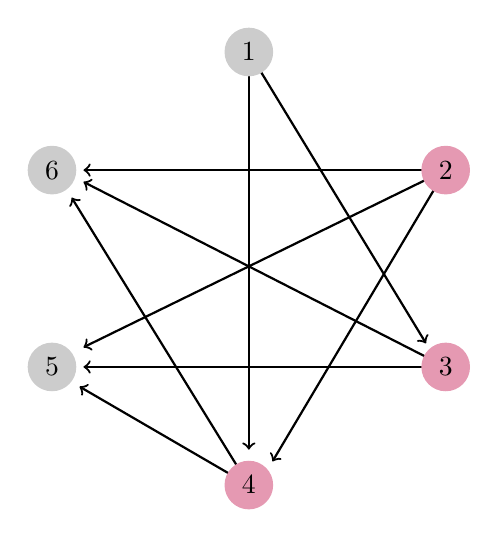
\begin{tikzpicture}[scale=0.5]
\draw[thick, ->] (5,13) -- (9.5,5.6);
\draw[thick, ->] (5,13) -- (5,2.9);
\draw[thick, ->] (10,10) -- (0.8,10);
\draw[thick, ->] (10,10) -- (0.8,5.5);
\draw[thick, ->] (10,10) -- (5.6,2.6);
\draw[thick, ->] (10,5) -- (0.8,5);
\draw[thick, ->] (10,5) -- (0.8,9.7);
\draw[thick, ->] (5,2) -- (0.7,4.5);
\draw[thick, ->] (5,2) -- (0.5,9.3);

\draw (5,13) node[circle,fill=black!20] {$1$};
\draw (10,10) node[circle,fill=purple!40] {$2$};
\draw (10,5) node[circle,fill=purple!40] {$3$};
\draw (5,2) node[circle,fill=purple!40] {$4$};
\draw (0,5) node[circle,fill=black!20] {$5$};
\draw (0,10) node[circle,fill=black!20] {$6$};

\end{tikzpicture} 
\caption[Network where node set $C = \{ 2,3 \}$ contests node $4$]{Network $D'$ where node set $C = \{ 2,3 \}$ contests node $4$}
\label{Complex Contestability}
\end{center}
\end{figure}

\noindent
Clearly, the coverage and reach of nodes $2$ and $3$ encapsulate the coverage of node $4$. Therefore, although nodes $2$ and $3$ do not contest node $4$ individually, the node set $C = \{ 2,3 \}$ contests node $4$. Indeed, the condition for group contestability holds:
\begin{equation}
P_{4}(D) \times S_{4}(D) \subset \left( \, \overline{P}_{2}(D - \{4\}) \times \overline{S}_{2}(D - \{4\}) \cup \overline{P}_{3}(D - \{4\}) \times \overline{S}_{3}(D - \{4\}) \, \right).
\end{equation}
If node $4$ is removed from the network its function can be fully replaced by the combination of nodes $2$ and $3$ and therefore all other nodes that were connected can still be connected in the same way.
\end{example}

Example~\ref{Group Contestability} highlights the requirement for $\overline{P}_{j}(D - \{i\})$ used in the definition of contestability instead of the predecessor set, $P_{j}(D - \{i\})$, only. Consider the network in Figure~\ref{Complex Contestability}. As noted, there exist no middlemen and all intermediaries are contested given the definition of contestability provided above. With a more restricted definition it would be seen that node $4$ would not be a contested intermediary and also not a middleman. The more elaborative version provided in Definition~\ref{Contested} adjusts for predecessors of a given node, $i$, that can connect to the successors of $i$, therefore fulfilling the same function and thus contesting $i$. 

Examples~\ref{Simple Contestability} and~\ref{Group Contestability} give an indication that if an intermediary is contested, it cannot be a middleman. For example, in Figure~\ref{weakmm} agent $3$ is a non-middleman because his function is directly contested by the presence of node $2$, and node $2$ is a middleman because its function is not contested by any other node in the network.

Our main result states that there is a duality between contestation and the presence of critical nodes.
\begin{theorem}[Duality of middlemen and contestability] \label{duality}
Consider any directed network $(N,D)$ with $n \geqslant 3$. Then:
\begin{itemize}
\item[(i)] Every middleman $i \in M(D)$ is uncontested.

\item[(ii)] If an intermediary $i \in N$ is uncontested, then it must be a middleman, i.e., $i \in M(D)$.
\end{itemize}
\end{theorem}
\begin{proof}
Let $(N,D)$ be a directed network with $n \geqslant 3$.
\smallskip\noindent
\emph{Proof of (i):}
The condition for contestability stated in equation (\ref{Group Contested}) on page \pageref{Group Contested} contends that a node $h \in N$ is contested in network $D$ if its coverage, determined by the nodes it intermediates, is a subset of the coverage and the reach of the nodes in $C_{h} \subset N \setminus \{ h \}$.
\\
Now consider an intermediary $i$ in $D$ that is contested by a set of agents, $C_{i} \subset N \setminus \{ i \}$. Since $i$ is contested, it must be true that all of $i$'s predecessors can be connected to all of $i$'s successors by a walk that does not include $i$. Therefore, $i$ cannot be a middleman. This implies the assertion that every middleman is uncontested.

\smallskip\noindent
\emph{Proof of (ii):}
Consider an intermediary $h \in N$ who is uncontested in the network $D$. Then $h$'s coverage is not a subset of the coverage of any set of nodes plus the respective reach of each of these nodes. This implies that $h$ itself has to rest on at least one walk that no other nodes in the network rest on when $h$ is removed from the network. Hence, in the network $D$ there exists at least one pair of nodes, say $i$ to $j$, with $h \in \cap \mathcal{W}_{ij} (D)$ and $\mathcal{W}_{ij}(D - \{h\}) = \varnothing$. This implies that $h$ is actually a middleman concerning the walks from $i$ to $j$.
\end{proof}

\medskip\noindent
From this assertion all middlemen are never contested; if a node is contested then all of its intermediation functions can be replaced by the coverage of other nodes. From this, it is contended that a middleman is an intermediary that has a unique function and is, in some way, more effective than non-middlemen with respect to their connectivity and thus coverage in the network.

\paragraph{Relationship with market competition.}

Considering an economic network in which all nodes produce an homogeneous output, the notion of contestability is linked to that of market competition. Traditional market theory contends that one agent competes against another if they produce the same output and subsequently sell this output to the same set of consumers. If two or more agents operate in a given market with access to the same set of suppliers and the same consumers, then all consumers could technically be supplied by another agent if one of the agents were removed from the network, or failed due to some exogenous shock.

Bertrand competition suggests that firms producing an homogenous output will be prone to compete with each other with respect to the price attached to their respective outputs \citep{Edgeworth1881}. Much of the analysis in market competition in economics has derived from this simple concept. Firms operating in this way will have no market power; potentially a price above the long-term marginal cost would be unsustainable since a competitor will be able to undercut it. Our notion of contestability is related to Bertrand competition in the sense that, if a given node is contested, its coverage and functions are contested, meaning that a contested node has no power in the network\footnote{Note that if all nodes provided a heterogeneous output then the notion of contestability and market competition breaks down. Furthermore, if we were to assume that all agents had highly differentiated information and ideas then individual nodes could technically not contest one another since they would all perform different functions and provide different insights into the network; indeed, all nodes will be unique.}.

\section{Measuring middleman power}
\label{networkpower}

A middleman occupies a critical position in a network since her removal disconnects at least two or more agents and, in the most extreme case, might have the ability to separate the network into multiple disconnected components. Therefore, it seems logical to ask how we can measure this power. After examining established measures, we propose a measure of middleman power based on the disconnections that emerge when middlemen are removed from the network.

\subsection{Betweenness centrality and middlemen}

We first examine whether betweenness centrality could be a tool to assess middleman power. \emph{Betweenness centrality} was proposed independently by \citet{Anthonisse1971} for edges and rephrased by \citet{Freeman1977} for nodes in undirected networks. \citet{White1994} proposed an extension to directed networks.

This measure seems specifically relevant since it explicitly considers the role of a node in connecting other nodes in the network. It may be expected that the betweenness centrality score of a node provides an indication of what nodes are middlemen by having a greater betweenness centrality than non-middlemen in the network.

To define the betweenness centrality measure, let $\pi(hj)$ be the number of shortest walks---or \emph{geodesics}---from node $h$ to node $j$. Furthermore, let $\pi_{i}(kj)$ be the number of geodesics that pass through node $i$. Betweenness centrality is now defined as

\begin{equation} \label{betweennesscentrality}
BC_{i}(D) = \sum_{h,j \neq i \colon \pi(hj) \neq 0} \frac{\pi_{i}(hj)}{\pi(hj)}
\end{equation}

Equation \ref{betweennesscentrality} indicates that a middleman $i$ between nodes $k$ and $j$ would always have a high betweenness centrality since by Definition~\ref{middleman} a middleman is on all walks between these two nodes. However, this formulation only considers geodesics. As the next example illustrates, the betweenness centrality of non-middlemen may even surpass that of middlemen.
\begin{example} \label{ex:BC}
Consider the acyclic directed network $D''$ depicted in Figure~\ref{mmnmm}.

\begin{figure}[h]
\begin{center}
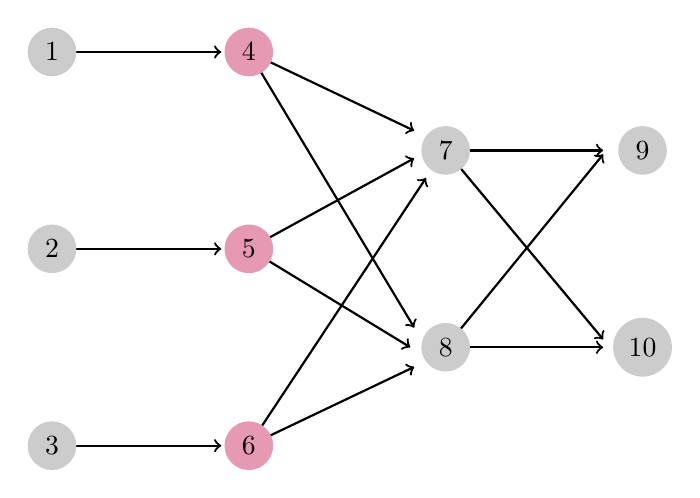
\begin{tikzpicture}[scale=0.5]
\draw[thick, ->] (0,10) -- (4.3,10);
\draw[thick, ->] (0,0) -- (4.3,0);
\draw[thick, ->] (0,5) -- (4.3,5);

\draw[thick, ->] (5,10) -- (9.2,8);
\draw[thick, ->] (5,10) -- (9.2,3);

\draw[thick, ->] (5,5) -- (9.2,7.3);
\draw[thick, ->] (5,5) -- (9.1,2.5);

\draw[thick, ->] (5,0) -- (9.5,6.8);
\draw[thick, ->] (5,0) -- (9.2,2);

\draw[thick, ->] (10,7.5) -- (14,7.5);
\draw[thick, ->] (10,2.5) -- (14,2.5);

\draw[thick, ->] (10,7.5) -- (14,2.7);
\draw[thick, ->] (10,2.5) -- (14,7.4);

\draw (0,0) node[circle,fill=black!20] {$3$};
\draw (0,5) node[circle,fill=black!20] {$2$};
\draw (0,10) node[circle,fill=black!20] {$1$};
\draw (5,0) node[circle,fill=purple!40] {$6$};
\draw (5,5) node[circle,fill=purple!40] {$5$};
\draw (5,10) node[circle,fill=purple!40] {$4$};
\draw (10,7.5) node[circle,fill=black!20] {$7$};
\draw (10,2.5) node[circle,fill=black!20] {$8$};
\draw (15,7.5) node[circle,fill=black!20] {$9$};
\draw (15,2.5) node[circle,fill=black!20] {$10$};

\end{tikzpicture}
\end{center}
\caption[Differentiating betweenness and middlemen]{The directed network $D''$ considered in Example~\ref{ex:BC}}
\label{mmnmm}
\end{figure}

\noindent Here $M(D'') = \{ 4, 5, 6 \}$, and nodes $7$ and $8$ are contested intermediaries. All middlemen have the same non-normalised betweenness centrality measures due to their equivalent positions: $BC_{4}(D'')=BC_{5}(D'')=BC_{6}(D'')=4$. However, both contested intermediaries have larger non-normalised betweenness centrality scores: $BC_{7}(D'')=BC_{8}(D'')=6$.

In the underlying undirected network, $U''$, where all arcs in $D''$ are reciprocated, the non-middlemen still have a higher betweenness centrality than middlemen: $BC_{4}(U'')=BC_{5}(U'')=BC_{6}(U'')=16.4$ and $BC_{7}(U'')=BC_{8}(U'')=25$. Table 2 provides a comparison of common centrality measures all of which indicate that nodes $7$ and $8$ are more central, therefore underrating the nodes with powerful middleman properties.
\end{example}

This deficiency concerning the identification and measure of middlemen, highlighted in Figure~\ref{mmnmm} and Table 2, extends to other less common centrality measures. Indeed, no measure for undirected networks specifically identifies and highlights middlemen, instead the measures tend to over-inflate the power and importance of contested intermediaries in networks.

The reason for the high betweenness centrality of non-middlemen, for example, is because of the underlying assumptions of the measure. First, only geodesic paths are counted between two given nodes, and the second is that these geodesic paths are considered to have an equal weight. The combination of these assumptions implies that the betweenness centrality measure does not necessarily measure the ``power'' of a node in negotiating between two others.

\begin{table}[t]
\begin{center}
\label{network2stats}
\begin{tabu}{ X[l] X[c] X[c] X[c] X[c] X[c] X[c]}

\\[-1.8ex]\hline
\hline \\[-1.8ex]
Node & Degree 	& PageRank	& Betweenness 	& Closeness 	& Bonacich 	& $\beta$-Measure\\ \hline
1    & 1    	& 0.112 	& 0.000    		& 0.360  		& 0.328 	& 0.333\\
2    & 1    	& 0.112 	& 0.000    		& 0.360  		& 0.328 	& 0.333\\
3    & 1    	& 0.112 	& 0.000    		& 0.360  		& 0.328 	& 0.333\\
4    & 3    	& 0.330 	& 0.456    		& 0.474  		& 1.047 	& 1.400\\
5    & 3    	& 0.330 	& 0.456    		& 0.474  		& 1.047 	& 1.400\\
6    & 3    	& 0.330 	& 0.456    		& 0.474  		& 1.047 	& 1.400\\
7    & 4    	& 0.480 	& 0.694    		& 0.692  		& 1.565 	& 2.000\\
8    & 4    	& 0.480 	& 0.694    		& 0.692  		& 1.565 	& 2.000\\
9    & 2    	& 0.297 	& 0.011    		& 0.474  		& 0.863 	& 0.400\\
10   & 2    	& 0.297 	& 0.011    		& 0.474  		& 0.863 	& 0.400\\ \hline
\end{tabu}\par
\caption{Centrality results for the undirected network $U''$}
\end{center}
\end{table}

\subsection{A middleman power measure}

We provide a mechanism to identify middlemen and quantify their brokerage power in a meaningful way from basic information regarding the topology of the network. The proposed measure counts the disconnections that emerge when a given node is removed from the network.

Let $D$ be a directed network on node set $N = \{1, \ldots ,n\}$ and let $i \in N$ be an arbitrary node. The \emph{brokerage} of node $i$ is quantified as

\begin{equation} \label{brokerage}
b_{i}(D) = \sum_{j \in N} \# S_{j}(D) - \sum_{j \neq i} \# S_{j}(D - \{i\}) - \#S_{i}(D) - \#P_{i}(D) .
\end{equation}

Note that the successor set of a node contains all other nodes that can be reached by a directed walk from the node. The first part of Equation \ref{brokerage}, $\sum_{j \in N} \# S_{j}(D)$, counts the total number of successors of all $n$ nodes in the network. Hence, it provides an indication of the total connectivity of the network as a whole.

Given the intuition of the first part of the equation, it can be implied that the second part, $\sum_{j \neq i} \# S_{j}(D - \{i\})$, refers to the total connectivity of the network when node $i$ is removed. We remark that $\sum_{j \in N} \# S_{j}(D) > \sum_{j \neq i} \# S_{j}(D - \{i\})$ if $d_{i}(D) \geqslant 1$, and $\sum_{j \in N} \# S_{j}(D) = \sum_{j \neq i} \# S_{j}(D - \{i\})$ if $d_{i} = 0$.

Thus, $\sum_{j \in N} \# S_{j}(D) - \sum_{j \neq i} \# S_{j}(D - \{i\})$ expresses the \emph{connectivity differential} between the full network $D$ and the subnetwork $D - \{i\}$. The connectivity differential captures two features: (1) The direct connectivity of node $i$ in terms of its successor and predecessor set. Indeed, the larger the predecessor and successor sets of node $i$ the larger the differential will be regardless of whether $i$ is a middleman or not. (2) The lost connectivity to other nodes not including $i$.

When considering the impact of a middleman, we are only interested in the lost connectivity (2) and, therefore, we compensate the connectivity differential with the connectivity of $i$ in the network. Specifically, the predecessor set and successor set of node $i$ is removed from the connectivity differential, thus adjusting for (1) and resulting in Equation~\ref{brokerage} above. The brokerage of a node therefore counts the number of third-party disconnections that occur due to the removal of a node; or in other words, counts the number of $(i,j)$-middleman sets that a node is a member of.

If $b_{i}(D) = 0$ then the removal of $i$ from the network makes no change to the network's connectivity---when compensating for the connectivity of $i$. Hence, all nodes that are connected by a directed walk in $D$ can still be connected in $D - \{i\}$. In essence, compensating for their connection to $i$ in $D$, the number of successors of all $j$ nodes is the same in $D - \{i\}$ as in $D$.

On the other hand, if $b_{i}(D) \geqslant 1$, there exists at least one pair of connected nodes that are now not connected in $D - \{i\}$, and $i$ must be a middleman.

\medskip\noindent We normalise the brokerage of a node by calculating the total number of potential opportunities for brokerage in the network. Brokerage---and, therefore, middleman positions---can only emerge if a pair of nodes are a minimum distance of two or more away from each other. Intuitively, by calculating the indirect successors of all nodes in the network, the total number of brokerage opportunities can be derived.

The set of indirect successors of $i$ in $D$ is given by $S_{i}(D) \setminus s_{i}(D)$. Therefore, the number indirect successors for node $i$ is given by $\# S_{i}(D) - \# s_{i}(D)$. Given this, the maximal potential brokerage in $D$ is computed as

\begin{equation} \label{normalisation}
B'(D) = \sum_{i \in N} \left[ \# S_{i}(D) - \# s_{i}(D) \right] .
\end{equation}

By normalising a node's brokerage score, the \emph{middleman power} of a node can be defined.

\begin{definition}[Middleman power] \label{middlemanpower}
Let $D$ be a directed network on node set $N$. The \textbf{middleman power} of node $i \in N$ is given as
\begin{equation} \label{mmpowerindex}
\nu_{i}(D) = \frac{b_{i}(D)}{B(D)} ,
\end{equation}
where $B(D) = \max \{ B'(D) , 1\}$.
\end{definition}

Empty and complete networks have to be assigned an artificial normalisation factor of unity as they would otherwise have no brokerage opportunities. 

A middleman has a network power of 1 if it brokers all potential opportunities in the network. This includes nodes at the centre of star networks; however, even if some of the leaf nodes form a connection between each other, the middleman power of the centre node remains 1.

The next example explicitly computes the middleman power for an undirected star and a directed cycle.

\begin{example} \label{starcycle}
For an arbitrary undirected star network, $D^{\star}$, where $n \geqslant 3$, $b_{i}(D^{\star}) = (n-1)(n-2)$ for the centre node, and $b_{j}(D^{\star})=0$ for all other nodes. The potential brokerage for an undirected star is computed as $B(D^{\star}) = (n-1)(n-2)$. Therefore, the middleman power of the centre node is
\begin{equation}
\nu_{i}(D^{\star}) = \frac{(n-1)(n-2)}{(n-1)(n-2)} = 1 .
\end{equation}

\noindent Next, consider a directed cycle $D^{\circ}$ for arbitrary $n\geqslant 3$. Each node has an in-degree of 1 and an out-degree of 1, implying that all nodes are middlemen. We now derive that $b_{1}(D^{\circ}) = \ldots = b_{n}(D^{\circ}) = \frac{(n-1)(n-2)}{2}$. The number of potential brokerage opportunities is $B (D^{\circ}) = n(n-2)$, implying $\nu_i = \frac{n-1}{2n}$ for all $i \in N$ where $n \geqslant 3$.
\end{example}

We derive several properties for the middleman power measure stated in (\ref{mmpowerindex}).

\begin{theorem} \label{middlemanpowert}
Let $D$ be a network on node set $N=\{1, \ldots ,n\}$.
\begin{abet}
\item[(i)] For any contested intermediary, $\nu_{i}(D) = 0$.
\item[(ii)] For any network $0 \leqslant \nu_{i} \leqslant 1$ for all $i \in N$.
\end{abet}
\end{theorem}

\begin{proof}
\emph{Proof of (i):}
Theorem~\ref{duality} asserts a duality between a contested intermediary and a non-middleman. Definition~\ref{middleman} implies that an intermediary $k$ is not a middleman if there is no pair $i,j \in N$ with $i \neq j$ such that $k$ lies on all walks from $i$ to $j$ in $D$. Hence, $k \notin \cap \mathcal{W}_{i,j}(D)$ for all $i,j \in N$ with $i \neq j$.
\\
Since $k$ is an intermediary it holds that $\# P_{k}(D) > 0$, $\# S_{k}(D) > 0$ as well as $\sum_{i \in N} \# S_{i}(D) > \sum_{i \in N \setminus \{k\}} \# S_{i}(D - \{k\})$ since the nodes in $D - \{k\}$ can obviously not connect to $k$. Also, since the connectivity of the network $D$ is not affected by the removal of node $k$, it holds that the removal of $k$ only affects the connectivity with $k$ itself. Hence, $\sum_{i \in N} \# S_{i}(D) - \sum_{i \in N \setminus \{k\}} \# S_{i}(D - \{k\}) = \# S_{k}(D) + \# P_{k}(D)$. Therefore, $b_k (D) =0$, implying that $\nu_{k} = 0$.
\\[1.5ex]
\emph{Proof of (ii):}
We omit a mathematical proof of (ii), due to its tedious nature. Instead, we provide an intuitive, more descriptive reasoning. 
\\
A middleman cannot take advantage of more than all brokerage opportunities present in a network; therefore $B'(D) \geqslant b_{i}(D)$, implying $\nu_{i}(D) \leqslant 1$\footnote{Only in a network where a middleman rests on all geodesic walks of length two, for example an undirected star, it holds that $B'(D) = b_{i}(D)$.}.
\\
Furthermore, neither $b_{i}(D) < 0$ nor $B(D) < 0$. The minimum brokerage of some node $k$ is in an empty network where $\# S_{k}(D) = \# P_{k}(D) = 0$. In that case, $\sum_{i \in N} \# S_{i}(D) = \sum_{i \neq k} \# S_{i}(D - \{k\})$ since $k$ has no connectivity in the network. Therefore, $\nu_i (D) \geqslant 0$ for any node $i \in N$.
\end{proof}

\medskip\noindent For large directed networks the calculation of the middleman power measure of a node can be tedious. The appendix to this paper contains a two-step algorithm based on the adjacency matrix of a directed network to identify middlemen and compute the middleman power measure of each node in an arbitrary directed network.

\subsubsection*{Distance-based brokerage}

We extend our discussion of the criticality of nodes with a measure that combines middleman power with node proximity. Consider a directed network $D$ on $N$ and $i,j,h \in N$ with $h \in M_{ij}(D)$. The brokerage power of middleman $h$ could be less effective due to the geodesic distance from $i$ to $j$.

Consider an amended brokerage score to capture this effect given by

\begin{equation}
\Delta_{ij}(h) = \frac{1}{\delta_{ih} \cdot \delta_{hj}},
\end{equation}
where $\delta_{ij}$ is the geodesic distance from $i$ to $j$ in $D$. Here, nodes closer to $h$ provide a greater brokerage power to node $h$ than those at larger distances. Indeed, $h$ receives maximal brokerage power if $i \in p_{h}(D)$ and $j \in s_{h}(D)$.

Now a \emph{distance based middleman power measure} for $h \in M(D)$ can be introduced as
\begin{equation}
\nu^{\ast}_h (D) = \sum_{i,j \in N \colon h \in M_{ij} (D)} \Delta_{ij} (h) .
\end{equation}

Reassessing the directed network in Figure~\ref{weakmm}, the distance-based middleman power measure provides a convergence of the middleman power scores for the nodes: $\nu^{\ast}_{6}(D) = 3 \frac{1}{3}$; $\nu^{\ast}_{5}(D) = 1 \frac{1}{2}$; $\nu^{\ast}_{2}(D) = 1$; $\nu^{\ast}_{1}(D) = \nu^{\ast}_{3}(D) = \nu^{\ast}_{4}(D) = \nu^{\ast}_{7}(D) = 0$.

It may be particularly beneficial to use this modified measure to assess costly trade in a network or the diffusion of information that can degrade as it is being passed through a network. This assumption of information degradation and even complete truncation over a certain distance has been widely used in literature regarding social networks \citep{JacksonRogers2005}.

\medskip \noindent We note that the middleman power measure should not be considered as a replacement for other centrality measures---it is itself not just a measure of centrality---rather it identifies a certain type of node in a network and measures brokerage. Instead, the measure can be complimented with other measures of centrality. The above example of distance-based brokerage is one of many augmentations that makes use of closeness centrality.

\section{Measuring competitiveness}

The competitiveness of a network is defined in terms of how much competition each individual player has on its functions. If a middleman exists in a network, then a conclusion can be drawn that the network is uncompetitive and resulting resource allocation can be highly distorted by powerful agents in exploitive positions. Moreover, the presence of more middlemen has the potential to be even more disruptive. If, on the other hand, all intermediary nodes are highly contested then it can be concluded that the network is competitive.

We measure the competitiveness of a network in two ways. First, we measure the competitiveness of a network in a static manner through the use of threshold sets and a derived notion of network thickness. Using these metrics the competitive state of each node can be determined by counting the minimum number of other nodes that need to be removed in order for the given node to become a middleman. By analysing how close each node is to becoming a middleman an indication for the competitiveness of the network becomes apparent. Secondly, we measure the competitiveness of a network in a dynamic manner. We discuss a complimentary notion of middleman robustness which measures how robust a middleman's exploitive position is to a change in the topology of the network; this in turn measures how easily other nodes can contest it.

\subsection{Threshold set}

The threshold set of some node, $i \in N$, reflects the number of other nodes that must be removed in order for $i$ to become a middleman. In essence the threshold set provides a measure for how contested the node is: the fewer the number of other nodes in a given nodes' threshold set, the less contested that node is, and the more potential power that an individual has. The threshold set of a node is defined as below.

\begin{definition}[Threshold set] \label{Threshold Set}
Let $D$ be a directed network on node set $N=\{1, \ldots, n\}$ with $n \geqslant 3$ and $i \in N$.

\begin{itemize} 
\item A node set $T_{i}(D) \subset N$ is a \textbf{threshold set} of the node $i$ if $i \in T_{i}(D)$, $1 \leqslant \# T_{i}(D) \leqslant n-2$ and node $i$ is a middleman in the subnetwork $D_{F_i}$, where $F_{i} = ( N \setminus T_{i}) \cup \{i\}$.

\item The \textbf{threshold environment} of node $i \in N$ is defined as the collection of all threshold sets of node $i$ given by 
\begin{equation}
\mathcal{T}_{i}(D) = \{T_{i} \mid T_{i} \subset N \mbox{ is a threshold set of } i \in N\}
\end{equation}
\item The \textbf{minimum threshold set} of $i$ is given by 
\begin{equation}
T_{i}^{\star}(D) = min \{ T_{i} \mid T_{i} \in \mathcal{T}_{i}(D)\}.
\end{equation}
There may exist a number of minimum threshold sets for a node, and therefore a set of minimum threshold sets is required, given as $\mathcal{T}_{i}^{\star}(D)$.
\end{itemize}
\end{definition}

The cardinality of a threshold set is between $1$ and $\infty$. If $T_{i} = \{i\}$ for some node $i \in N$ then $i \in \mathcal{M}(D)$, and if $T_{i} = \varnothing$ then we set $\# T_{i} = \infty$ meaning that $i$ can never be middleman. Example~\ref{5node} below illustrates the concept of a threshold set.

\begin{figure}[t]
\begin{center}
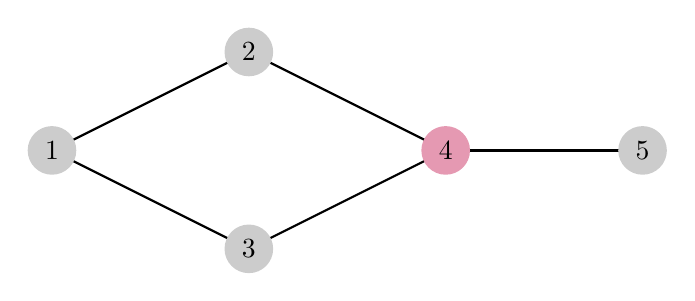
\begin{tikzpicture}[scale=0.5]
\draw[thick] (0,2.5) -- (5,5);
\draw[thick] (0,2.5) -- (5,0);
\draw[thick] (5,5) -- (10,2.5);
\draw[thick] (5,0) -- (10,2.5);
\draw[thick] (10,2.5) -- (15,2.5);

\draw (0,2.5) node[circle,fill=black!20] {$1$};
\draw (5,5) node[circle,fill=black!20] {$2$};
\draw (5,0) node[circle,fill=black!20] {$3$};
\draw (10,2.5) node[circle,fill=purple!40] {$4$};
\draw (15,2.5) node[circle,fill=black!20] {$5$};

\end{tikzpicture}
\end{center}
\caption{Undirected network $D$ with a strong middleman}
\label{Fig:5node}
\end{figure}

\begin{example} \label{5node}
Consider the network $D$ on the node set $N= \{1,2,3,4,5\}$ depicted in Figure~\ref{Fig:5node}. In this network $\mathcal{M}(D) = \{4\}$ which brokers all relations to and from node 5. The threshold environments of the network are given as follows:
\begin{align*}
&\mathcal{T}_{1}(D) = \{14, 145\}\\
&\mathcal{T}_{2}(D) = \{23, 235\}\\
&\mathcal{T}_{3}(D) = \{23, 235\}\\
&\mathcal{T}_{4}(D) = \{4, 14, 24, 34, 124, 134, 145\}\\
&\mathcal{T}_{5}(D) = \varnothing .
\end{align*}
Since node $4$ is already a middleman, it is itself a threshold set. Node $5$ can never be a middleman since it is a leaf node.
\end{example}

The notion of a threshold set is closely linked to the notion of contestability. By definition all threshold sets cannot be contested: if there exists a collection of nodes that contest a threshold set, then the threshold set would not be a threshold set. We state a Theorem below that links the concepts of a threshold set and contestation.

\begin{theorem}
Let $D$ be a network on node set $N$, where $i \in N$. If $T_{i}(D) \setminus \{i\} \neq \varnothing$ then the set $T_{i}(D) \neq \{i\}$ at least partially contests $i$.  
\end{theorem}

A number of propositions can be made regarding the concept of threshold sets, these are noted below.

\begin{proposition}
Let $D$ be some connected network on the node set $N$. Then the following properties must hold.

\begin{abet}
\item[(i)] All minimum threshold sets are symmetric in the sense that if $T^{\star} \in \mathcal{B}_{i}(D)$ for some $i \in N$, then for every node $j \in T^{\star} \colon T^{\star} \in T_{j}(D)$.

\item[(ii)] If $n \geqslant 3$ and the network $D$ is incomplete in the sense that $\# D < n(n-1)$, then for at least one node $i \in N$ it holds that $\mathcal{T}_{i}(D) \neq \varnothing$, i.e., $i$ has at least one threshold set.

\item[(iii)] For the complete network $D_{N}$ and every node $i \in N \colon \mathcal{T}_{i} (D_{N}) = \varnothing$.

\item[(iv)] Let $n > 3$. If node $i \in N$ is a leaf in the network $D$ with $d_{i}(D) = 1$, then $\mathcal{T}_{i}(D) = \varnothing$.

\item[(v)] For every node $i \in N \colon \mathcal{T}_{i} (D) = \varnothing$ if $d_{i} \leqslant 1$ or $\mathfrak{C}_{i}=1$.
\end{abet}
\end{proposition}

The notion of a threshold set forms the basis of a simple index that measures the power of a node in a network. This power index indicates how many competitors a node has in a given network.

\subsection{Network thickness}

Above we introduced an index that reflects how many competitors a certain individual has within a network. The fewer competitors, the more power an individual has. The smallest threshold set of an individual $i \in N$ in a network $D$ is that case that $\{i\} \in T_{i}^{\star}(D)$. This corresponds to the case where $i$ is a middleman in the network $D$.

Here we introduce a metric that measures the number of competitors that an individual has within a given network. The index is zero if there are no competitors that an individual has within a given network. The index is maximal if the individual is completely powerless and can never be in a powerful position regardless of which nodes are removed from the network. This metric is termed as the 

\begin{definition}[Thickness index]
Let $D$ be a network on node set $N$ where $\# N \geqslant 3$ and $i \in N$ is some node.

\begin{abet}
\item[(a)] The \textbf{thickness index} of the node $i$ in network $g$ is defined as
\[ 
\tau_{i}(g) = \left\{ \begin{array}{ll}
              \min \{\# T_{i} \mid T_{i} \in \mathcal{T}_{i}(D)\} - 1 & \mbox{if $\mathcal{T}_{i}(g) \neq \varnothing$}\\
         	 \infty & \mbox{if $\mathcal{T}_{i}(g) = \varnothing$}.\end{array} \right. 
\]
\item[(b)] The \textbf{network thickness index} of $D$ is defined as
\begin{equation*}
\tau(D) = \min \{ \tau_{i}(D) \mid i \in N \} . 
\end{equation*}
\end{abet}
\end{definition}

The thickness index indicates the competitiveness that a node is facing in the context of her network environment. A lower thickness index indicates fewer competitors and, therefore, a higher potential to attain power. The lowest thickness index of zero implies that the given node has no competitors and is a middleman.

\begin{definition}[Network thickness]
Let $D$ be a network on node set $N=\{1, \ldots, n\}$. If $\mathcal{M}(D) = \varnothing$ then the network $D$ is \textbf{thick}. If $\mathcal{M}(D) \neq \varnothing$ then the network $D$ is \textbf{thin}, meaning that all nodes have some competition attached.
\end{definition}

A network has a thickness index of zero if and only if it contains at least one middleman. Conversely, a network as a thickness index of 1 or more if all nodes are contested by at least one other node.

How contested an individual is is particularly important for the dynamic perception of competition and contestability. If all nodes are contested middlemen then if a single node is removed at random a middleman would inevitably appear. Moreover, within a social or economic context, there is more diversity when nodes are increasingly contested. Indeed, there are many alternative walks and pathways that trade, ideas, and information can flow through, and therefore diversity exists within the network. Characteristics of the thickness index are given below:

\begin{proposition}
Let $D$ be some network on node set $N$ and let $i \in N$ be some node. Then the following properties hold.

\begin{abet}

\item[(i)] If $\tau_{i}(D) \neq \infty$, then $\tau_{i}(g) \leqslant n-3$.

\item[(ii)] The node $i$ is a middleman in $D$ if and only if $\tau_{i}(D) = 0$.

\item[(iii)] The network $D$ contains a middleman if and only if $\tau_{i}(D) = \infty$.

\item[(iv)] Every leaf node $i$ of network $D$ has $\tau_{i}(D)=\infty$.

\item[(v)] If node $i$ has perfect clustering $\mathfrak{C}_{i}(D) = 1$, then $\tau_{i}(D) = \infty.$

\item[(vi)] The network is thick if and only if it has thickness index $\tau(g) \geqslant 1$.
\end{abet}
\end{proposition}

The relationship between thickness and clustering is interesting; it is natural to realise that networks with high clustering rarely have middlemen and that if a node is removed from a triad, no remaining nodes can become middlemen.

There is an immediate problem with the measure of thickness above. The problem is that even if the network only has one middleman the thickness will be rendered as zero regardless of how much more competition there is in the network. The measure misses a lot of other information about the topology of the network.

Is there a way to measure instead the thickness of all nodes in the network that have the potential to be middlemen divided by the maximal thickness of a node in the network that is not infinity. So, given a network of $n$ nodes the maximal thickness of each node will be $n-3$.

\subsection{Middleman robustness}

The exploitive position of a middleman can have varying levels of \emph{robustness} irrespective of its power. We perceive middleman robustness to infer how a given node can maintain an exploitive position even when there is a shock to the structure of the network due to the addition or deletion of arcs, links or nodes. There are a number of ways in which to measure the robustness of a given middleman. We provide three ways in which to measure middleman robustness: the first two measures assess the robustness of a nodes exploitive position given the deletion and addition of arcs; and the third assess middleman robustness given the removal of nodes from the initial network.

It is stipulated that a more robust middleman position is less sensitive to a change in the structure of the network. As social and economic relationships are formed between existing nodes, a middleman will be more prone to losing its powerful position if it is less robust. It is worth noting that the measurement of robustness is not easily applicable to networks that remain static over long periods of time such as neural and biological networks, nor networks in which individual nodes do not have autonomy to add or remove arcs and links such as technological infrastructures. However, the measure is directly applicable to social and economic networks where the structure can be highly volatile.

\subsubsection{Link robustness measures}

The \emph{$\alpha$-robustness} of a middleman is defined as the minimum number of arcs that need to be formed in the network in order for a middleman to be completely circumvented by all predecessors, and therefore lose its middleman position. From this we note the dual of $\alpha$-robustness, given as $\gamma$-robustness, which measures the minimum number of links that have to be removed from the network such that a given middleman loses its brokerage power.

\begin{definition}[$\alpha$- and $\gamma$-robustness measures] \label{robustness}
Let $D$ be some network on node set $N = \{1,\ldots,n\}$ where $i \in \mathcal{M}(D) \subseteq N$. 
\begin{itemize}
\item[(a)] The \textbf{$\alpha$-robustness} of $i$ is given by:
\begin{equation} 
\alpha_{i} = \min \, \left\{ \, \# D' \mid D \subset D' \mbox{ and } i \notin \mathcal{M}(D') \, \right\} - \# D , 
\end{equation}
where $\# D' > \# D$.

\item[(b)] The \textbf{$\gamma$-robustness} of $i$ is given by:
\begin{equation} 
\alpha_{i}^{\star} = \# D - \max \, \left\{ \# D' \mid D' \subset D \mbox{ and } i \notin \mathcal{M}(D) \, \right\} , 
\end{equation} 
where $\# D' < \# D$.
\end{itemize}
\end{definition}

In our case $D$ refers to the the set of arcs in a network, therefore the cardinality of $D$ provides a figure for the number of arcs in the network. The $\alpha$-robustness of a middleman is clearly given as the minimum number of arcs that need to be added to the initial network $D$ in order for a middleman to be completely circumvented and subsequently lose its position as a middleman. The dual of the $\alpha$-robustness is the $\gamma$-robustness which measures the minimum number of arcs that need to be removed from the initial network $D$ such that a given middleman no longer has an exploitive position in the resulting network $D' \subset D$.

If a node is a middleman then the value of both the $\alpha$-robustness and the $\gamma$-robustness will always be a positive integer. However, neither of the robustness measures will necessarily be correlated with its middleman power, in many situations there can exist an increasing middleman power with a constant $\alpha$-robustness and $\gamma$-robustness.

An alternative way in which to interpret the $\alpha$-robustness measure is based on how easily a middleman can be contested by sets of other nodes. A low value for $\alpha_{i}$ means that it takes few relationships to be activated in order for a given middleman, $i$, to be contested. We would consider a relatively small network to have low values of $\alpha$ for all middlemen. Finally it is worth noting that the $\alpha$-robustness is always finite and bounded by $(n-1)$ and $\gamma$-robustness is also always finite and bounded by $\min \{ \# s_{i}, \# p_{i} \}$. 

\subsubsection{Node robustness measure}

The $\beta$-robustness of a middleman is an extension of the $\gamma$-robustness measure. The $\beta$-robustness of a middleman is defined in terms of the minimum number of nodes that need to be deleted in order for a given node to lose its middleman position.

\begin{definition}[$\beta$-robustness measure]
Let $D$ be a network on node set $N$ and let $D'$ be a network on node set $N'$ where $N' \subset N$. There exists some node $i \in N' \cap N$ such that $i \in \mathcal{M}(D)$. The \textbf{$\mathbf{\beta}$--robustness} of node $i$ is given as:
\begin{equation}
\beta_{i} = \# N - \max \, \{ \, \# N' \mid N' \subset N \mbox{ and } i \notin \mathcal{M}(D') \, \} . 
\end{equation}
\end{definition}

Much like before, if a node is a middleman then the $\beta$-robustness of the node will always be a finite positive integer bounded by $n-2$, however the measure is not necessarily positively correlated with the middleman power of the node. An extension of the $\beta$-robustness measure is to assume that node deletion is based on some probability distribution.

\medskip \noindent A result from the assessment of middleman power and robustness is that there can emerge cases in which middlemen with an extremely high middleman power can have a low robustness. If this is so then it is either easily circumvented or it can easily lose its position if there are shocks to the network that lead it to losing nodes. Given this, a low robustness means that irrespective of the middleman power of the node there is a large opportunity for it to become contested or not an intermediary.

The middleman power of a node provides a good indication of its robustness, however it is not necessarily true that a higher middleman power indicates a higher robustness. A higher middleman power provides a greater potential for having a larger robustness. A higher middleman power allows for the potential for a higher complexity in the middleman's predecessor and successor set. Indeed, the robustness of the middleman is increased if a greater number of its successors require the presence of the middleman to be connected to each other, and likewise for its predecessors.


\section{An application to two empirical networks}

In this section we apply our two middleman power measures to two well-known social networks. From the assessment of these networks we provide a discussion regarding the potential of middlemen in these networks. The results of middleman power are compared with other measures of centrality. This is done in terms of reference; we refrain from correlating the results of these measures because we showed above that middleman power measures different aspects of a node than other measures.

\subsection{The elite Florentine marriage network}

The investigation of the marriage network of renaissance Florence has been extensively used to assess the effectiveness of many centrality measures to highlight positions of importance and influence \citep{Newman2003betweenness}. Following from our discussion of the House of Medici to introduce our notion of entrepreneurship in chapter~\ref{ch:entrepreneurship}, and the socio-economic networks shown there, we apply our analysis of critical nodes to this network as well.

\begin{figure}[t]
\centering
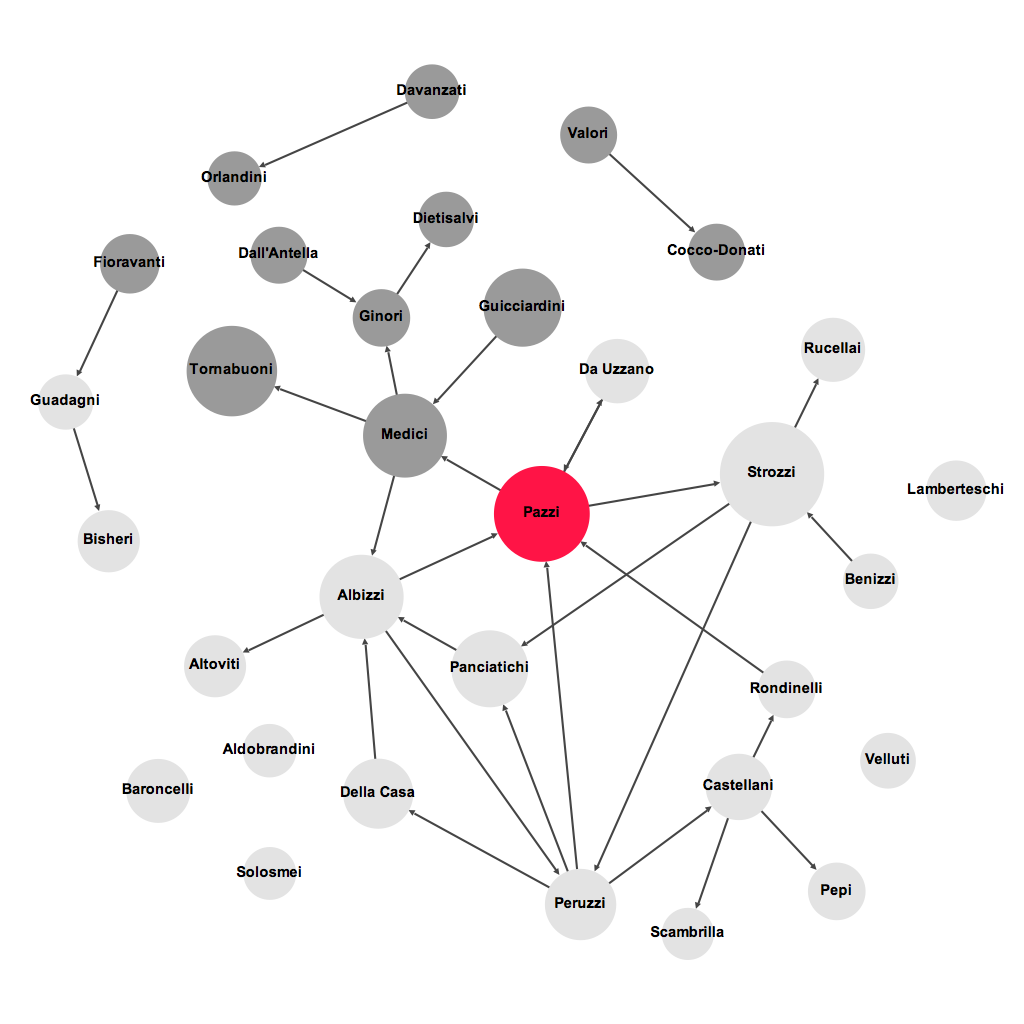
\includegraphics[scale=0.37]{imgs/Florentine-marr.png}
\caption{Directed network of Florentine marriages (c. 1434)}
\label{Fig:FlorentineFamilies}
\end{figure}

It has been shown in contemporary studies of the marriage network that the Medici family have the highest degree, closeness, and betweenness centralities. However, \citet{Roover1963}, \citet{Padgett1994} and \citet{Goldthwaite2009} explain that their importance and power in the marriage network especially is derived from their ability to access diverse sources of information between separate factions of the Florentine elite and subsequently broker relationships between families of separate factions. As such, the Medici family filter information by allowing or not allowing pieces of information to spread to other factions; thus largely monopolising informational spread. Powerful brokerage opportunities, which the Medici took advantage of, emerged due to the inherent ``network disjunctures within the elite'' \citep[p.~1259]{Padgett1993}. In particular, \citet{Padgett1993} show that Cosimo de'Medici was able to gain access to, and control, the flow of diverse information between opposing political factions and also between families in the same faction. Thus, a middleman position allowed the Medici family to attain power within Florentine society; especially, the Medici's ability to act as broker between a large number of families crossing opposing political factions.

Unlike more recent renditions of the Florentine marriage network where the marriage network is depicted as a reduced undirected graph---but keeping in line with the format initially provided by \citet[p.~1276--1277]{Padgett1993}---we represent this network as a directed graph. In doing so we draw an arc from family $i$ to family $j$ to represent a female from family $i$ married into family $j$. The resulting marriage network can be seen in Figure~\ref{Fig:FlorentineFamilies}\footnote{The data was initially gathered by \citet{Kent1978} and a blockmodel network was constructed and used in \citet{Padgett1993} and \citet{Padgett1994}. The network provided in Figure~\ref{Fig:FlorentineFamilies} is derived from these studies. Both provide an extremely rich analysis of the elite in Florence at this time.}. The intuition for this representation is that families were strategically married in order to build trust, inherit wealth, property, and business, as well as influence the political and economic decisions of other families. Information will have flowed through these relationships and these marriage will have often supported economic relationships in the form of trade, employment and loan provision. Moreover, unlike more recent assessments of the Florentine marriage network we include families as groups; thus all nodes represent a group of families under the same name. The groups of families are coloured depending on the factions that the families were affiliated: dark grey nodes are families affiliated with the Medician faction; light grey nodes are families affiliated with the opposing Oligarch faction; and the only family with clear split loyalties (which became increasingly oligarchical over time) is the Pazzi family coloured in red. Finally the size of the node corresponds to the relative cumulative gross wealth of the family in the group: a node of a relatively large size is considered to have a relatively large gross wealth. For reference, the node of the smallest size is the Scambrilla family.

Data was gathered regarding the cumulative gross wealth of groups of all families. This data can be derived from the census and property survey of Florentine dominions in the province of Tuscany, 1427--1480. The data has also been posted online as the \emph{Online Catasto of 1427} and can be found in Appendix B of \citet{Padgett1993}. The Medici family, despite their political and cultural prominence, are only considered as the fifth wealthiest elite family in Florence during this time. The Medici are not even the wealthiest family in their own faction; they are second to the Tornabuoni family. This information expresses two features: first, this was not the zenith period of the Medici; and second, it can be argued that it was specifically the Medici's superior position in the marriage network as opposed to just their economic presence that allowed them to gain command in Florence during this time. Elaborating on the first point we note that although the Medici had established a considerable banking dynasty by 1427 it was still under the command of Giovanni di'Bicci de'Medici. We know from  It wasn't until the reign of Cosimo di'Giovanni de'Medici in 1929 that the House of Medici rose to phenomenal economic and political prominence. The argument made by the second point provides the basis for our discussion regarding the structure of the network and the centrality of families with respect to the strategic marriages.

\subsubsection{Network structure}

There are 11 families in the Medician faction and 21 families in the oligarchic faction. The marriage network contains 9 weakly connected components and 23 strongly connected components. The giant weakly connected component contains 62.5\% of all elite families in the analysis. The network diameter is 6 with an average path length of 2.881 and the directed network density is 0.031. The average degree is 0.969, and the distribution is similar to that of a power law. The maximal $k$-core is 4 and contains the Pazzi, Peruzzi, Strozzi, and Albizzi families: these families form a \emph{rich club}. The network thickness index is 0.

A non-technical analysis of the network produced in Figure~\ref{Fig:FlorentineFamilies} highlights a clear distinction between the connectivity of the two main factions. If we were to include the Pazzi as a member of the Oligarch faction then only $\frac{3}{31}$ of the marriages formed were marriages between families of different factions. It is also clear that the families of the Pazzi, Albizz and Madici are clear gate-keepers to information flows between the factions within the main component. However, the Medici is the only family that acts as a (strong) middleman between both factions; the removal of the Medici leads to the partitioning of the factions in the main component.

The structure of the Medician faction takes the form of a rooted tree---a hierarchical construct---where the Medici family exist at the root. Such a structure provides a better basis for top-down organisation and the distribution of command throughout the elite families. This structure contrasts with the Oligarchic faction where individual agents are more densely connected and thus more structurally equivalent. It was explained that the Oligarchic faction suffered from ill-defined leadership and inter-faction power struggles. This more decentralised structure is certainly reflected in the marriage network. Specifically, \citet{Padgett1993} and \citet{PadgettMcLean2006} noted that the Oligarchic faction was less cohesive and more disorganised than the Medician faction. From our analysis it is seen that there are more brokerage opportunities in the Oligarchic faction highlighting that they were more disjunctured. We see that $\tfrac{7}{16}$ of the connected Oligarchs are middlemen against $\tfrac{2}{11}$ of the families in the Medician faction. Thus, the presence of more middleman positions within the Oligarchs decentralised structure allows for more brokering of information flows and, as such, a greater ability to manipulate information flows between members of the faction. This potential for the manipulation of information derived from the positional attributes of a family was not as prominent a feature within the Medician faction.

Further, we note that when running Newman's Q-measure of network modularity \citep{Newman2004detecting, Newman2006}---which gives the value of 0.521---the different factions can be easily partitioned. More specifically, Oligarchic faction is deconstructed into three distinct communities whereas the Medician faction remains as one district community. Moreover, the partitioning of the communities are determined by the middlemen within the faction. This measure of modularity reinforces the disjunctured nature of the Oligarchic faction. The community structure of the giant weakly connected component can be seen in Figure~\ref{Fig:Florentinemodu} in the appendices of this chapter.

\subsubsection{Centrality and power}

We analyse the resulting directed network in Figure~\ref{Fig:FlorentineFamilies} in a more technical way using in-degree $\left(d^-\right)$, out-degree $\left(d^+\right)$, \citet{Bonacich1987} eigenvector centrality ($E$), betweenness centrality ($BC$), and the normalised middleman power ($\nu$) of each family. The results of the analysis on middlemen is presented in Table~\ref{tabFlorence}. A full table of centrality analysis can be found in Table~\ref{tabFlorenceA} in the appendices of this chapter. In both tables the (*) and (**) after the family's name denotes a weak middleman and strong middleman. Throughout the analysis below we discuss the centrality and power of a family in both the directed and undirected network.

\begin{table}
\begin{center}
\begin{tabu} to \textwidth {X[l]  X[c]  X[c]  X[c]  X[c]  X[c]}
\\[-1.8ex]\hline
\hline \\[-1.8ex]
	            & Gross   &								 &			 &		   &		  \\
Name 		    & wealth  & $d^+_i$ $\left(d^-_i\right)$ & $BC_i$    & $E_i$   & $\nu_i$  \\ \hline
Albizzi(**)     & 249,940 & 3(3) 						 & 0.066 	 & 0.701   & 0.357 	  \\
Castellani(**)  & 111,355 & 3(1) 						 & 0.034 	 & 0.310   & 0.187 	  \\
Ginori(**)      & 42,333  & 1(2) 						 & 0.014 	 & 0.257   & 0.076    \\
Guadagni(**)    & 25,179  & 1(1) 						 & 0.001 	 & 0.001   & 0.006 	  \\
Medici(**)      & 248,105 & 3(2) 						 & 0.058 	 & 0.506   & 0.269 	  \\
Pazzi(**)       & 341,198 & 3(4) 						 & 0.093 	 & 1.000   & 0.503    \\
Peruzzi(*)      & 150,375 & 4(2) 						 & 0.070 	 & 0.612   & 0.287    \\
Rondinelli(*)   & 43,588  & 1(1) 						 & 0.014 	 & 0.157   & 0.076    \\
Strozzi(**)     & 407,296 & 3(2) 						 & 0.053 	 & 0.506   & 0.152    \\ \hline
\end{tabu}%\par
\caption{Analysis of middlemen in the elite marriage network of Renaissance Florence}
\label{tabFlorence}
\end{center}
\end{table}

The simplest measurement of the centrality and power of a node is the number of links it has in a network. In a directed network the connections that a node has can be partitioned into the number of direct successors (node out-degree) and the number of direct predecessors (node in-degree). The Peruzzi family has the greatest number of direct successors (4) and the Pazzi have the greatest number of direct predecessors (4); the Pazzi family also have the greatest sum of direct successors and direct predecessors (7). In an undirected network the connections that a node has is simply the total number of links that a node has; this is not necessarily the same as the sum of direct predecessors and direct successors as some node may be both a direct predecessor and direct successor. If the network were transformed to its undirected form then the Pazzi, the Albizzi, and Peruzzi families are connected to 6 families each. The Medici and Strozzi families are connected to 5 families each. 

There are two aspects to note from the assessment of node degree. First we note that, in general, families with a relatively higher degree are more prone to be middlemen in the network. This is true for most families apart from the Guadagni who are conveniently positioned such that their single in-degree and single out-degree forms a middleman position. Second, we note that the Medici faction does not have the highest degree centrality relative to other families in the Oligrahic faction.

Assessing the marriage network with the middleman power index highlights the Medici family as a strong middleman, along with the prominent Albizzi, Castellani, Ginori, Pazzi, and Strozzi families. It is, however, the Pazzi and Albizzi families that have a greater middleman power (0.503 and 0.357, respectively) than the Medici (0.269). The diversity of the Medici's brokered relationships extend further than those of the Albizzi and Pazzi families as the Medici brokers between factions. If, however, the direct marriage network is transformed into an undirected network such that information can flow in both directions then the Medici becomes the most powerful middleman with a normalised middleman power of 0.470; they are followed by the Ginori, Castellani and Strozzi families who have a normalised middleman power of 0.213. if the marriage network were converted into its undirected form, the Medici retains its strong middleman position maintaining the highest middleman power in the marriage network, and therefore control the flow of information and influence between more families.

The betweenness centrality measure ranks the Pazzi family as the most central in the directed marriage network. The measure favours middlemen thus typically ranking them higher; eight out of the top ten families in terms of their betweenness score are either weak or strong middlemen. In the undirected representation of the network the Medici have the highest betweenness centrality (0.166) followed by the Pazzi (0.142).

Unsurprisingly, the Bonacich centrality measure also ranks the Pazzi family highly, but also ranks many non-middlemen highly; specifically the Panciatichi family. From the network topology alone there is no indication to suggest that the Panciatichi family should have had a prominent role in the Florentine elite. Although the Medici rank highly with this measure, the relevance of an eigenvector centrality measure is questionable: there is no real reason to believe why the importance of a family would come from its degree and the degree of its neighbours alone. However, despite that the eigenvector centrality correlates highly with the gross wealth of the 

\subsubsection{Threshold sets, thickness and middleman robustness}

Due to the low density of the directed marriage network only one elite family---the Panciatichi family---is a non-middleman that can potentially become a middleman from the removal of other families in the network. Specifically, given the removal of the Peruzzi family the Panciatichi family becomes a middleman in the directed network. The Panciatichi family therefore has a thickness of 1. All other nodes either have a thickness of 0, since they can never be a middleman, or a thickness of $\infty$, since they already are middlemen.

We finally discuss the robustness of each middleman position in terms of the $\alpha$-robustness, $\beta$-robustness, and $\gamma$-robustness measures that were developed in this chapter. We provide information on the robustness of middlemen in both the directed and undirected marriage networks and the results can be seen in Table~\ref{FlorenceRobust}. In general we find that the $\beta$- and $\gamma$-robustness measures provide extremely similar results. The directed network highlights the Albizzi and Pazzi families as being robust; especially in terms of the $\beta$-robustness and $\gamma$-robustness measures. Both families are followed by the Medici, who are substantially robust across all measures. The results of the robustness measures suggests that there is a clear distinction between the consistency of some middlemen over others. All robustness measurements provide the same result with respect the the undirected form of the marriage network. The Medici is highlighted as being the most robust strong middleman in the undirected network. Notably, even though the Pazzi and Albizzi were robust in the directed network they both perform poorly in terms of the undirected representation of the marriage network.

\begin{table}[]
\centering
\begin{tabu} to \textwidth {X[l]  X[c]  X[c]  X[c] || X[c]  X[c]  X[c]  X[c]} 
\hline \hline
               &              & Directed    &              &              & Undirected  &              \\
Name           & $\alpha_{i}$ & $\beta_{i}$ & $\gamma_{i}$ & $\alpha_{i}$ & $\beta_{i}$ & $\gamma_{i}$ \\ \hline
Albizzi(**)    & 6            & 3           & 3            & 1            & 1           & 1            \\
Castellani(**) & 3            & 1           & 1            & 2            & 2           & 2            \\
Ginori(**)     & 2            & 1           & 1            & 2            & 2           & 2            \\
Guadagni(**)   & 1            & 1           & 1            & 1            & 1           & 1            \\
Medici(**)     & 6            & 2           & 2            & 3            & 3           & 3            \\
Pazzi(**)      & 6            & 3           & 3            & 1            & 1           & 1            \\
Peruzzi(*)     & 2            & 2           & 2            & 0            & 0           & 0            \\
Rondinelli(*)  & 1            & 1           & 1            & 0            & 0           & 0            \\
Strozzi(**)    & 4            & 2           & 2            & 2            & 2           & 2            \\ \hline
\end{tabu}
\caption{Robustness analysis of middlemen in Renaissance Florence}
\label{FlorenceRobust}
\end{table}

The robustness and centrality measures do not highlight the factions that exist within this network, and therefore simply assumes that relationships can be made without social or institutional pressures. As a consequence it could be argued that, regardless of the robustness measures, the Medici has the highest middleman robustness due to the fact that they are middlemen across both factions. Indeed, social and marriage relationships cannot be formed so seamlessly between families of opposing factions, therefore the robustness of the Medici's position is further strengthened due to the institutional pressures of society itself. This is, as previously discussed, a convincing reason for why the Medici's powerful position was stable for such a long time.

\medskip\noindent The Medici attained control in Florence because they not only brokered relationships between elite families in the network, but because they brokered relationships between two opposing factions. Therefore, they were not only able to gather and intercept information between the factions but also use it to their advantage. This is the prerogative of middlemen in social networks; to not only intercept and facilitate information between agents, but to manipulate and exploit it.

\begin{figure}[t]
\centering
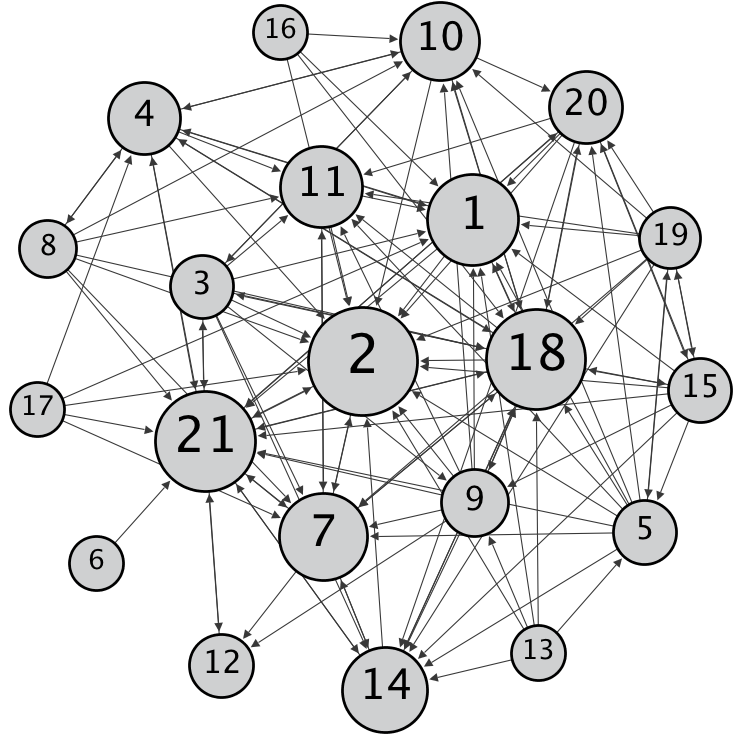
\includegraphics[scale=0.45]{imgs/krack.png}
\caption{Krackhardt's network of advice among managers}
\label{krackhardtnetwork}
\end{figure}

\subsection{Middlemen in Krackhardt's advice network}

Next we consider an example of a well-known organisational advice network in which \citet{Krackhardt1987} investigated the relationships between managers in a given firm\footnote{We use data in the ``LAS'' matrix from p.~129 in the Krackhardt article as it seems to be the most objective measure.}. He considered an organisation of about 100 employees and 21 managers. Krackhardt collected information from the managers about who sought advice from whom, depicted in Figure~\ref{krackhardtnetwork} on page \pageref{krackhardtnetwork}. An arc from $i$ to $j$ denotes that manager $i$ has sought advice from manager $j$; therefore, an arc from $j$ to $i$ denotes that manager $j$ has provided advice to manager $i$. In this depiction the size of the node reflects its in-degree.

\begin{table}[h]
\begin{center}
\begin{tabu} to \textwidth {X[l]  X[c]  X[c]  X[c]  X[c]  X[c]}

\\[-1.8ex]\hline
\hline \\[-1.8ex]
Manager       & $d^-_i$ $\left(d^+_i\right)$& $E_i$    & $BC_i$   & $\nu_i$  & $\nu_{i}^{*}$\\ \hline
1             & 12 (4)           & 0.068    & 0.035    & 0.000    & 0.000		 \\
2             & 18 (2)           & 0.306    & 0.011    & 0.000    & 0.000		 \\
3             & 3 (9)            & 1.271    & 0.018    & 0.000    & 0.000		 \\
4(*)          & 6 (7)            & 1.001    & 0.071    & 0.090    & 0.034		 \\
5             & 3 (10)           & 1.463    & 0.009    & 0.000    & 0.000		 \\
6             & 0 (1)            & 0.172    & 0.000    & 0.000    & 0.000		 \\
7             & 11 (6)           & 0.776    & 0.048    & 0.000    & 0.000		 \\
8             & 1 (7)            & 1.013    & 0.001    & 0.000    & 0.000		 \\
9             & 4 (9)            & 1.171    & 0.011    & 0.000    & 0.000		 \\
10            & 8 (5)            & 0.820    & 0.018    & 0.000    & 0.000		 \\
11            & 9 (3)            & 0.344    & 0.004    & 0.000    & 0.000		 \\
12            & 3 (1)            & 0.172    & 0.000    & 0.000    & 0.000		 \\
13            & 0 (6)            & 0.938    & 0.000    & 0.000    & 0.000		 \\
14            & 10 (4)           & 0.625    & 0.002    & 0.000    & 0.000		 \\
15(*)         & 3 (9)            & 1.265    & 0.092    & 0.161    & 0.064		 \\
16            & 0 (4)            & 0.580    & 0.000    & 0.000    & 0.000		 \\
17            & 0 (5)            & 0.673    & 0.000    & 0.000    & 0.000		 \\
18            & 15 (12)          & 1.745    & 0.231    & 0.000    & 0.000		 \\
19            & 2 (10)           & 1.493    & 0.002    & 0.000    & 0.000		 \\
20            & 6 (7)            & 1.028    & 0.028    & 0.000    & 0.000		 \\
21(**)        & 15 (8)           & 1.348    & 0.176    & 0.147    & 0.051		 \\ \hline
\end{tabu}
\caption{Influence, centrality, and middlemen in Krackhardt's advice network}
\label{tabkrackhardt}
\end{center}
\end{table}

In Table 4, using the same centrality measures as before, we identify two weak middlemen, managers 4 and 15, and one strong middleman, manager 21\footnote{As before, (*) indicates a weak middleman and (**) indicates a strong middleman.}. Middlemen are important for this network for a number of intuitive reasons: First, a middleman can block ideas, advice, and information from being transmitted from one group of managers to another. Second, a middleman can manipulate the information transferred from one group of managers to another.

The weak middleman, manager (node) 15, has the highest brokerage in the organisation controlling a total of 34 relationships. This is also reflected in that \citet{Krackhardt1987} highlighted manager 15 as an important agent in the organisational advice network. However, Node 15 does not have the highest betweenness or Bonacich centralities. Instead, Node 18 is the most prominent in terms of Bonacich and betweenness scores but is not a middleman in the network; instead this may be a function of the in- and out-degree of node 18.

Both Bonacich and betweenness centralities are also seen to be poor indicators for ranking middlemen: Node 15 is the most powerful middleman in the network, but has a Bonacich and betweenness centrality lower than Node 21. The Bonacich influence model does not consider the fact that middlemen are potentially able to exploit their position by using information from others and blocking the transmission of certain information and ideas.

\subsubsection{Concluding comments}

Due to the formation of new socio-economic roles entrepreneurial agents can assume unique positions in a network. These unique positions can intuitively be seen with respect to their connectivity in the socio-economic space and can be defined accurately as middleman positions. Positioning oneself in a unique way in the socio-economic space is the essence of a network entrepreneur as discussed in Chapter~\ref{ch:entrepreneurship}. 

Middlemen possess an ability to connect pairs of agents who would otherwise be disconnected from each other; these can have liberating externalities for those directly or indirectly connected to middlemen in the form of opening new exchange routes and channels of information, but middlemen can exploit their position and as such act in a highly extractive way to their neighbourhood. Whether a middleman behaves in an exploitive or facilitating manner is ambiguous and dependent on the institutional environment; however the middleman power measure provides a mechanism in which to measure the positional power of the middleman and therefore provides an objective quantitative value to the potentially extractive or value-generating nature of the entrepreneurial agent.

The assessment of middlemen is purely individualised. We can extend the assessment to collective economic interaction and thus cooperative economic activities to include coalitions of economic agents who as a whole form a middleman position in a network.


\begin{subappendices}

\section{Power and centrality in Renaissance Florence networks} 
\label{A}

This chapter analysed the network structure and node centrality of elite Florentine marriages. Here we provide more information as to the modularity of the network (Figure~\ref{Fig:Florentinemodu}) and centrality of nodes within the network (Table~\ref{tabFlorenceA}).

\begin{figure}[h!]
\centering
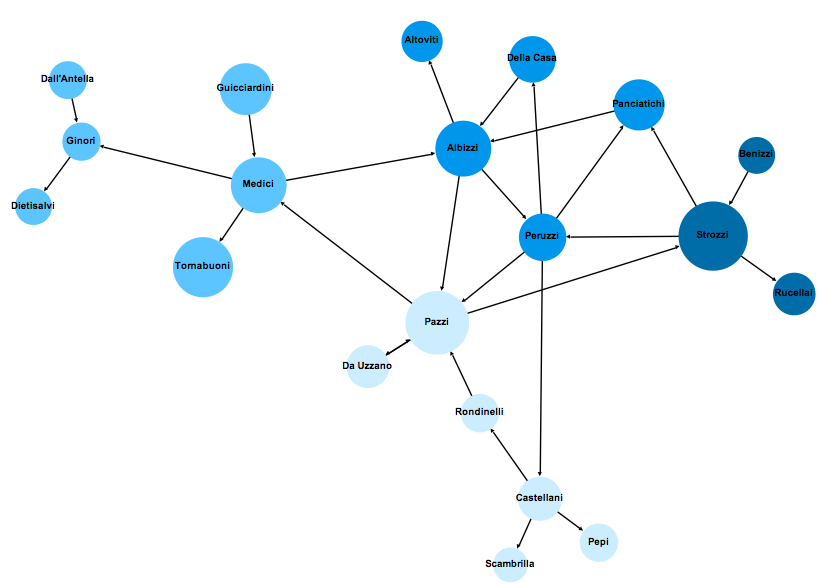
\includegraphics[scale=0.4]{imgs/Florentine-modu.png}
\caption{Community structure detection on elite Florentine marriages}
\label{Fig:Florentinemodu}
\end{figure}

\begin{table}
\begin{center}
\begin{tabu} to \textwidth {X[l]  X[r]  X[c]  X[c]  X[c]	X[c]  X[c]}
\\[-1.8ex]\hline
\hline \\[-1.8ex]
          & Gross  &  &  &  & \\
Family 			    & wealth & $d^+_i$ $\left(d^-_i\right)$   	&  $BC_i$		&  $E_i$		&  $\nu_i$        \\ \hline
Albizzi(**)     & 249,940 & 3(3) & 0.066 & 0.701 & 0.357      \\
Aldobrandini    & 10,805  & 0(0) & 0.000 & 0.000 & 0.000      \\
Altoviti        & 77,621  & 0(1) & 0.000 & 0.355 & 0.000      \\
Baroncelli      & 92,615  & 0(0) & 0.000 & 0.000 & 0.000      \\
Benizzi         & 26,093  & 1(0) & 0.000 & 0.000 & 0.000      \\
Bisheri         & 78,729  & 0(1) & 0.000 & 0.002 & 0.000      \\
Castellani(**)  & 111,355 & 3(1) & 0.034 & 0.310 & 0.187      \\
C-Donati        & 37,260  & 0(1) & 0.000 & 0.001 & 0.000      \\
Da Uzzano       & 96,131  & 1(1) & 0.000 & 0.506 & 0.000      \\
Dall'Antella    & 37,914  & 1(0) & 0.000 & 0.000 & 0.000      \\
Davanzati       & 19,887  & 1(0) & 0.000 & 0.000 & 0.000      \\
Della Casa      & 140,624 & 1(1) & 0.001 & 0.309 & 0.000      \\
Dietisalvi      & 26,274  & 0(1) & 0.000 & 0.132 & 0.000      \\
Fioravanti      & 57,674  & 1(0) & 0.000 & 0.000 & 0.000      \\
Ginori(**)      & 42,333  & 1(2) & 0.014 & 0.257 & 0.076      \\
Guadagni(**)    & 25,179  & 1(1) & 0.001 & 0.001 & 0.006      \\
Guicciardini    & 203,087 & 1(0) & 0.000 & 0.000 & 0.000      \\
Lamberteschi    & 64,775  & 0(0) & 0.000 & 0.000 & 0.000      \\
Medici(**)      & 248,105 & 3(2) & 0.058 & 0.506 & 0.269      \\
Orlandini       & 16,315  & 0(1) & 0.000 & 0.001 & 0.000      \\
Panciatichi     & 193,878 & 1(2) & 0.005 & 0.566 & 0.000      \\
Pazzi(**)       & 341,198 & 3(4) & 0.093 & 1.000 & 0.503      \\
Pepi            & 43,100  & 0(1) & 0.000 & 0.157 & 0.000      \\
Peruzzi(*)      & 150,375 & 4(2) & 0.070 & 0.612 & 0.287      \\
Rondinelli(*)   & 43,588  & 1(1) & 0.014 & 0.157 & 0.076      \\
Rucellai        & 93,891  & 0(1) & 0.000 & 0.256 & 0.000      \\
Scambrilla      & 148     & 0(1) & 0.000 & 0.157 & 0.000      \\
Solosmei        & 5,757   & 0(0) & 0.000 & 0.000 & 0.000      \\
Strozzi(**)     & 407,296 & 3(2) & 0.053 & 0.506 & 0.152      \\
Tornabuoni      & 299,878 & 0(1) & 0.000 & 0.257 & 0.000      \\
Valori          & 37,842  & 1(0) & 0.000 & 0.000 & 0.000      \\
Velluti         & 28,108  & 0(0) & 0.000 & 0.000 & 0.000      \\ \hline
\end{tabu}%\par
\caption{Measuring the importance of Florentine families (c. 1434)}
\label{tabFlorenceA}
\end{center}
\end{table}

\end{subappendices}